\ifx\wholebook\relax \else
% ------------------------ 

\documentclass{article}
%------------------- Other types of document example ------------------------
%
%\documentclass[twocolumn]{IEEEtran-new}
%\documentclass[12pt,twoside,draft]{IEEEtran}
%\documentstyle[9pt,twocolumn,technote,twoside]{IEEEtran}
%
%-----------------------------------------------------------------------------
%%
% loading packages
%
\newif\ifpdf
\ifx\pdfoutput\undefined % We're not running pdftex
  \pdffalse
\else
  \pdftrue
\fi
%
%
\ifpdf
  \RequirePackage[pdftex,%
            CJKbookmarks,%
       bookmarksnumbered,%
              colorlinks,%
          linkcolor=blue,%
              hyperindex,%
        plainpages=false,%
       pdfstartview=FitH]{hyperref}
\else
  \RequirePackage[dvipdfm,%
             CJKbookmarks,%
        bookmarksnumbered,%
               colorlinks,%
           linkcolor=blue,%
               hyperindex,%
         plainpages=false,%
        pdfstartview=FitH]{hyperref}
  \AtBeginDvi{\special{pdf:tounicode GBK-EUC-UCS2}} % GBK -> Unicode
\fi
\usepackage{hyperref}

% other packages
%-----------------------------------------------------------------------------
\usepackage{graphicx, color}
\usepackage{CJK}
%
% for programming 
%
\usepackage{verbatim}
\usepackage{listings}


\lstdefinelanguage{Smalltalk}{
  morekeywords={self,super,true,false,nil,thisContext}, % This is overkill
  morestring=[d]',
  morecomment=[s]{"}{"},
  alsoletter={\#:},
  escapechar={!},
  literate=
    {BANG}{!}1
    {UNDERSCORE}{\_}1
    {\\st}{Smalltalk}9 % convenience -- in case \st occurs in code
    % {'}{{\textquotesingle}}1 % replaced by upquote=true in \lstset
    {_}{{$\leftarrow$}}1
    {>>>}{{\sep}}1
    {^}{{$\uparrow$}}1
    {~}{{$\sim$}}1
    {-}{{\sf -\hspace{-0.13em}-}}1  % the goal is to make - the same width as +
    %{+}{\raisebox{0.08ex}{+}}1		% and to raise + off the baseline to match -
    {-->}{{\quad$\longrightarrow$\quad}}3
	, % Don't forget the comma at the end!
  tabsize=2
}[keywords,comments,strings]

\lstloadlanguages{C++, Lisp, Smalltalk}

% ======================================================================

\def\BibTeX{{\rm B\kern-.05em{\sc i\kern-.025em b}\kern-.08em
    T\kern-.1667em\lower.7ex\hbox{E}\kern-.125emX}}

\newtheorem{theorem}{Theorem}

%
% mathematics
%
\newcommand{\be}{\begin{equation}}
\newcommand{\ee}{\end{equation}}
\newcommand{\bmat}[1]{\left( \begin{array}{#1} }
\newcommand{\emat}{\end{array} \right) }
\newcommand{\VEC}[1]{\mbox{\boldmath $#1$}}

% numbered equation array
\newcommand{\bea}{\begin{eqnarray}}
\newcommand{\eea}{\end{eqnarray}}

% equation array not numbered
\newcommand{\bean}{\begin{eqnarray*}}
\newcommand{\eean}{\end{eqnarray*}}

\RequirePackage{CJK,CJKnumb,CJKulem,CJKpunct}
% we use CJK as default environment
\AtBeginDocument{\begin{CJK*}{GBK}{song}\CJKtilde\CJKindent\CJKcaption{GB}}
\AtEndDocument{\clearpage\end{CJK*}}

%
% loading packages
%
\newif\ifpdf
\ifx\pdfoutput\undefined % We're not running pdftex
  \pdffalse
\else
  \pdftrue
\fi
%
%
\ifpdf
  \RequirePackage[pdftex,%
       bookmarksnumbered,%
              colorlinks,%
          linkcolor=blue,%
              hyperindex,%
        plainpages=false,%
       pdfstartview=FitH]{hyperref}
\else
  \RequirePackage[dvipdfm,%
        bookmarksnumbered,%
               colorlinks,%
           linkcolor=blue,%
               hyperindex,%
         plainpages=false,%
        pdfstartview=FitH]{hyperref}
\fi
\usepackage{hyperref}

% other packages
%-----------------------------------------------------------------------------
\usepackage{graphicx, color}
%
% for programming 
%
\usepackage{verbatim}
\usepackage{listings}
\usepackage{algorithmic} %for pseudocode
\usepackage{algorithm}


\lstdefinelanguage{Smalltalk}{
  morekeywords={self,super,true,false,nil,thisContext}, % This is overkill
  morestring=[d]',
  morecomment=[s]{"}{"},
  alsoletter={\#:},
  escapechar={!},
  literate=
    {BANG}{!}1
    {UNDERSCORE}{\_}1
    {\\st}{Smalltalk}9 % convenience -- in case \st occurs in code
    % {'}{{\textquotesingle}}1 % replaced by upquote=true in \lstset
    {_}{{$\leftarrow$}}1
    {>>>}{{\sep}}1
    {^}{{$\uparrow$}}1
    {~}{{$\sim$}}1
    {-}{{\sf -\hspace{-0.13em}-}}1  % the goal is to make - the same width as +
    %{+}{\raisebox{0.08ex}{+}}1		% and to raise + off the baseline to match -
    {-->}{{\quad$\longrightarrow$\quad}}3
	, % Don't forget the comma at the end!
  tabsize=2
}[keywords,comments,strings]

\lstloadlanguages{C++, Lisp, Haskell, Python, Smalltalk}

% ======================================================================

\def\BibTeX{{\rm B\kern-.05em{\sc i\kern-.025em b}\kern-.08em
    T\kern-.1667em\lower.7ex\hbox{E}\kern-.125emX}}

\newtheorem{theorem}{Theorem}

%
% mathematics
%
\newcommand{\be}{\begin{equation}}
\newcommand{\ee}{\end{equation}}
\newcommand{\bmat}[1]{\left( \begin{array}{#1} }
\newcommand{\emat}{\end{array} \right) }
\newcommand{\VEC}[1]{\mbox{\boldmath $#1$}}

% numbered equation array
\newcommand{\bea}{\begin{eqnarray}}
\newcommand{\eea}{\end{eqnarray}}

% equation array not numbered
\newcommand{\bean}{\begin{eqnarray*}}
\newcommand{\eean}{\end{eqnarray*}}




\setcounter{page}{1}

\begin{document}

\fi
%--------------------------

% ================================================================
%                 COVER PAGE
% ================================================================

\title{Divide and conquer, Quick sort V.S. Merge sort}

\author{Liu~Xinyu
\thanks{{\bfseries Liu Xinyu } \newline
  Email: liuxinyu95@gmail.com \newline}
  }

\markboth{Quick sort V.S. Merge sort}{AlgoXY}

\maketitle

\ifx\wholebook\relax
\chapter{Divide and conquer, Quick sort V.S. Merge sort}
\numberwithin{Exercise}{chapter}
\fi

% ================================================================
%                 Introduction
% ================================================================
\section{Introduction}
\label{introduction} 

It's proved that the best approximate performance of comparison based sorting is $O(N \lg N)$ \cite{TAOCP}.
In this chapter, two divide and conquer sorting algorithms are introduced. Both of them
perform in $O(N \lg N)$ time. One is quick sort. It is
the most popular sorting algorithm. Quick sort has been well studied, many programming libraries provide
sorting tool based on quick sort. 

In this chapter, we'll first introduce the idea of of quick sort, which demonstrates the power of divide 
and conquer strategy well. Several variants will be explained, and we'll see when quick sort performs poor
in some special cases. That the algorithm is not able to partition the sequence in balance.

In order to solve the unbalanced partition problem, we'll next introduce about merge sort, which ensure
the sequence to be well partitioned in all the cases. Some variants of merge sort, including nature merge
sort, bottom-up merge sort are shown as well.

Similar as other chapters, all the algorithm will be realized in both imperative and functional approaches.

% ================================================================
% Quick sort
% ================================================================
\section{Quick sort}
\index{Quick sort}

Consider a teacher arranges a group of kids in kindergarten to stand in a line for some game.
The kids need stand in order of their heights, that the shortest one stands on the left most,
while the tallest stands on the right most. How can the teacher instruct these kids, so that
they can stand in a line by themselves?

\begin{figure}[htbp]
 \centering
 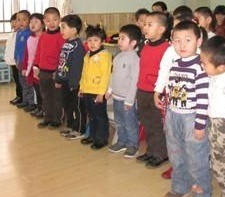
\includegraphics[scale=0.8]{img/kids-inline.eps}
 \caption{Instruct kids to stand in a line}
 \label{fig:knuth-ssort}
\end{figure}

There are many strategy, and the quick sort approach can be applied here:

\begin{enumerate}
  \item The first kid raises his/her hand. The kids who are shorter than him/her stands to the left to this child; the kids who are taller than him/her stands to the right of this child;
  \item All the kids move to the left if there are repeat the above step; all the kids move to the right repeat the same step as well.
\end{enumerate}

Suppose a group of kids with their heights as $\{102, 100, 98, 95, 96, 99, 101, 97\}$ with [cm] as the unit. 
The following table illustrate how they stand in order of height by folllowing this method.

\begin{tabular}{ | c c c c c c c c |}
\hline
{\bf 102} & 100 & 98 & 95 & 96 & 99 & 101 & 97 \\
{\bf 100} & 98 & 95 & 96 & 99 & 101 & 97 & {\em 102} \\
{\bf 98} & 95 & 96 & 99 & 97 & {\em 100} & 101 & {\em 102} \\
{\bf 95} & 96 & 97 & {\em 98} & 99 & {\em 100} & {\em 101} & {\em 102} \\
{\em 95} & {\bf 96} & 97 & {\em 98} & {\em 99} & {\em 100} & {\em 101} & {\em 102} \\
{\em 95} & {\em 96} & 97 & {\em 98} & {\em 99} & {\em 100} & {\em 101} & {\em 102} \\
{\em 95} & {\em 96} & {\em 97} & {\em 98} & {\em 99} & {\em 100} & {\em 101} & {\em 102} \\
\hline
\end{tabular}

At the beginning, the first child with height 102 cm raises his/her hand. We call this kid the pivot and mark
his height in bold.
It happens that this is the tallest kid.
So all others stands to the left side, which is represented in the second row of above table. Note that
the child with height 102 cm is in the final ordered position, thus we mark it italic. Next the kid with
height 100 cm raise hand, so the children of heights 98, 95, 96 and 99 cm stand to his/her left, and there
is only 1 child of height 101 cm who is taller than this pivot kid. So he stands to the right hand.
The 3rd row in the table shows this stage accordingly. After that, the child of 98 cm high is seleced
as pivot on left hand; while the child of 101 cm high on the right is selected as pivot. Since there
are no other kids in the unsorted group with 101 cm as pivot, this small group is ordered already and
the kid of height 101 cm is in the final proper postion. The same method is applied to the group of kids
which haven't been in correct order until all of them are stands in the final position.

\subsection{Basic version}
Summarize the above insruction leads to the recursive description of quick sort. In order to sort a sequence
of elements $L$.

\begin{itemize}
\item If $L$ is empty, the result is obviously empty; This is the trivial edge case;
\item Otherwise, select an arbitrary element in $L$ as a pivot, recursively sort all elements not greater than $L$, put
the result on the left hand of the pivot, {\em and} recursively sort all elements which are greater than $L$, put
the result on the right hand of the pivot.
\end{itemize}

Note that the emphasized word {\em and}, we don't use `then' here, which indicate it's quite OK that 
the recursive sort on the left and right can be done in parrallel. We'll return this parallism topic soon.

Quick sort was first developed by C. A. R. Hoare in 1960 \cite{TAOCP}, \cite{wiki-qs}. What we describe here
is a basic version. Note that it doesn't state how to select the pivot. We'll see soon that the pivot selection
affects the performance of quick sort later.

The most simple method to select the pivot is always choose the first one so that quick sort can be formalized 
as the following.

\be
sort(L) = \left \{
  \begin{array}
  {r@{\quad:\quad}l}
  \Phi & L = \Phi \\
  sort(\{ x | x \in L', x \leq l_1 \} \cup \{ l_1 \} \cup sort(\{ x | x \in L', l_1 < x \}) & otherwise \\
  \end{array}
\right.  
\ee

Where $l_1$ is the first element of the non-empty list $L$, and $L'$ contains the rest elements $\{l_2, l_3, ...\}$.
Note that we use Zermelo Frankel expression (ZF expresssion for short), which is also known as list
comprehension. A ZF expression $\{ a | a \in S, p_1(a), p_2(a), ... \}$ means take all element in set $S$,
if it satisfies the predication $p_1, p_2, ...$. The result is also a list. Please refer to the appendix
about list in this book for detail.

It's quite straightforward to translate this equation to real code if list comprehension is supported.
The following Haskell code is give for example:

\lstset{language=Haskell}
\begin{lstlisting}
sort [] = []
sort (x:xs) = sort [y | y<-xs, y <= x] ++ [x] ++ sort [y | y<-xs, x < y]
\end{lstlisting}

This might be the shortest quick sort program in the world at the time when this book is written. Even
a verbose version is still very expressive:

\lstset{language=Haskell}
\begin{lstlisting}
sort [] = []
sort (x:xs) = as ++ [x] ++ bs where
    as = sort [ a | a <- xs, a <= x]
    bs = sort [ b | b <- xs, x < b]
\end{lstlisting}

There are some variants of this basic quick sort program, such as using explicit filtering instead of
list comprehension. The following Python program demonstrates this for example:

\lstset{language=Python}
\begin{lstlisting}
def sort(xs):
    if xs == []:
        return []
    pivot = xs[0]
    as = sort(filter(lambda x : x <= pivot, xs[1:]))
    bs = sort(filter(lambda x : pivot < x, xs[1:]))
    return as + [pivot] + bs
\end{lstlisting}

\subsection{Strict weak ordering}
We assume the elements are sorted in monotonic none decreasing order so far. It's quite possible to customize
the algorithm, so that it can sort the elements in other ordering criteria. This is necessary in practice because
users may sort numbers, strings, or other complex objects (even list of lists for example) and so on.

The typical generic solution is to abstract the comparison as a parameter as we mentioned in chapters about 
insertion sort and selection sort. Although it needn't the total ordering, the comparison must satisfy 
{\em strict weak ordering} at least \cite{wiki-total-order} \cite{wiki-sweak-order}.

For the sake of brevity, we only considering sort the elements by using less than or equal 
(equivelent to not greater than) in the rest of the chapter.

\subsection{Partition}
\index{Quick sort!partition}
Observing that the basic version actually takes two passes to find all elements not greater than the pivot and 
the rest. Such partition can be accomplished by only one pass. We explicitly define the partition as below.

\be
partition(p, L) = \left \{
  \begin{array}
  {r@{\quad:\quad}l}
  (\Phi, \Phi) & L = \Phi \\
  (\{ l_1 \} \cup A, B) & p(l_1), (A, B) = partition(p, L') \\
  (A, \{ l_1 \} \cup B) & \lnot p(l_1)
  \end{array}
\right.  
\ee

Note that the operation $\{x\} \cup L$ is just a `cons' operation, which only takes constant time.
The quick sort can be modified accordingly.

\be
sort(L) = \left \{
  \begin{array}
  {r@{\quad:\quad}l}
  \Phi & L = \Phi \\
  sort(A) \cup \{l_1\} \cup sort(B) & otherwise, (A, B) = partition(\lambda_x x \leq l_1, L')
  \end{array}
\right.  
\ee

Translating this new algorithm into Haskell yields the below code.

\lstset{language=Haskell}
\begin{lstlisting}
sort [] = []
sort (x:xs) = sort as ++ [x] ++ sort bs where
    (as, bs) = partition (<= x) xs

partition _ [] = ([], [])
partition p (x:xs) = let (as, bs) = partition p xs in
    if p x then (x:as, bs) else (as, x:bs)
\end{lstlisting}

The concept of parition is very cirtical to quick sort. Partition is also very important to many
other sort algorithms. We'll explain how it generally affects the sorting methodology by the end
of this chapter. Before further discussion about fine tuning of quick sort specific partition, let's
see how to realize it in-place imperatively.

There many partition methods. The one given by Nico Lomuto \cite{pearls} \cite{CLRS} will be used here as it's
easy to understand. We'll show other partition algorithm soon and see how it affects the performance.

\begin{figure}[htbp]
   \centering
   \subfloat[Partition invariant]{\includegraphics[scale=0.5]{img/partition-1-way.ps}} \\
   \subfloat[Start]{\includegraphics[scale=0.5]{img/partition-1-way-start.ps}} \\
   \subfloat[Finish]{\includegraphics[scale=0.5]{img/partition-1-way-finish.ps}}
   \caption{Partition a range of array by using the left most element as pivot.} 
   \label{fig:partition-1-way}
\end{figure}

Figure \ref{fig:partition-1-way} shows the idea of this one-pass partition method. The array is processed from
left to right. At any time, the array consists of the following parts as shown in figure \ref{fig:partition-1-way} (a): 

\begin{itemize}
\item The left most cell contains the pivot; By the end of the partition process, the pivot will be moved to the 
final proper position;
\item A segment contains all elements which are not greater than the pivot. The right boundary of this segment is
marked as `left';
\item A segment contains all elements which are greater than the pivot. The right boundary of this segment is marked
as `right'; It means that elements between `left' and `right' marks are greater than the pivot;
\item The rest of elements after `right' marks haven't been processed yet. They may greater than the
pivot or not.
\end{itemize}

At the beginning of partition, the `left' mark points to the pivot and the `right' mark points to the 
the second element next to the pivot in the array as in Figure
\ref{fig:partition-1-way} (b); Then the algorithm repeatedly advances the right mark one elements after the other
till pass the end of the array. 

In every iteration, the element pointed by the `right' mark is compared with the
pivot. If it is greater than the pivot, it should be among the segment between the `left' and `right' marks, so that
the algorithm goes on to advance the `right' mark and examine the next element; Otherwise, since the element pointed
by `right' mark is less than or equal to the pivot (not greater than), it should be put before the `left' mark.
In order to achieve this, the `left' mark needs be advanced by one, then exchange the elements pointed by the `left' 
and `right' marks.

Once the `right' mark passes the last element, it means that all the elements have been processed. The elements 
which are greater than the pivot have been moved to the right hand of `left' mark while the others are to the
left hand of this mark. Note that the pivot should move between the two segments. An extra exchanging between the pivot and
the element pointed by `left' mark makes this final one to the correct location. This is shown by the swap 
bi-directional arrow in figure \ref{fig:partition-1-way} (c).

The `left' mark (which points the pivot finally) partitions the whole array into two parts, it is 
returned as the result. We typically increase the `left' mark by one, so that it points to the
first element greater than the pivot for convinient. Note that the array is modified in-place.

The partition algorithm can be described as the following. It takes three arguments, the array $A$, the lower
and the upper bound to be partitioned \footnote{The partition algorithm used here is slightly different from
the one in \cite{CLRS}. The latter uses the last element in the slice as the pivot.}.

\begin{algorithmic}[1]
\Function{Partition}{A, l, u}
  \State $p \gets A[l]$  \Comment{the pivot}
  \State $L \gets l$ \Comment{the left mark}
  \For{$R \in [l+1, u)$} \Comment{iterate on the right mark}
    \If{$\lnot (p < A[R])$} \Comment{negate of $<$ is enough for strict weak order}
      \State $L \gets L + 1$
      \State \textproc{Exchange} $A[L] \leftrightarrow A[R]$
    \EndIf
    \State \textproc{Exchange} $A[L] \leftrightarrow p$
  \EndFor
  \State \Return $L + 1$ \Comment{The parition position}
\EndFunction
\end{algorithmic}

Below table shows the steps of paritioning the array $\{ 3, 2, 5, 4, 0, 1, 6, 7\}$.

\begin{tabular}{ | c c c c c c c c | l |}
\hline
(l) {\bf 3} & (r) 2 & 5 & 4 & 0 & 1 & 6 & 7 & initialize, $pivot = 3, l = 1, r = 2$ \\
{\bf 3} & (l) 2 & (r) 5 & 4 & 0 & 1 & 6 & 7 & $5 > 3$, moves on \\
{\bf 3} & (l) 2 & 5 & (r) 4 & 0 & 1 & 6 & 7 & $4 > 4$, moves on \\
{\bf 3} & (l) 2 & 5 & 4 & (r) 0 & 1 & 6 & 7 & $0 < 3$ \\
{\bf 3} & 2 & (l) 0 & 4 & (r) 5 & 1 & 6 & 7 & Advances $l$, then swap with $r$ \\
{\bf 3} & 2 & (l) 0 & 4 & 5 & (r) 1 & 6 & 7 & $1 < 3$ \\
{\bf 3} & 2 & 0 & (l) 1 & 5 & (r) 4 & 6 & 7 & Advances $l$, then swap with $r$ \\
{\bf 3} & 2 & 0 & (l) 1 & 5 & 4 & (r) 6 & 7 & $6 > 3$, moves on \\
{\bf 3} & 2 & 0 & (l) 1 & 5 & 4 & 6 & (r) 7 & $7 > 3$, moves on \\
1 & 2 & 0 & 3 & (l+1) 5 & 4 & 6 & 7 & $r$ passes the end, swap pivot and $l$ \\
\hline
\end{tabular}

This version of partition algoritm can be implemented in ANSI C as the following.
\lstset{language=C}
\begin{lstlisting}
int partition(Key* xs, int l, int u) {
    int pivot, r;
    for (pivot = l, r = l + 1; r < u; ++r)
        if (!(xs[pivot] < xs[r])) {
            ++l;
            swap(xs[l], xs[r]);
        }
    swap(xs[pivot], xs[l]);
    return l + 1;
}  
\end{lstlisting}

Where \verb|swap(a, b)| can either be defined as function or a macro. In ISO C++, \verb|swap(a, b)|
is provided as a function template. the type of the elements can be defined somewhere or abstracted
as a template parameter in ISO C++. We omit these language specific details here.

With the in-place partition realized, the imperative in-place quick sort can be accomplished by using it.

\begin{algorithmic}[1]
\Procedure{Quick-Sort}{$A, l, u$}
  \If{$l < u$}
    \State $m \gets$ \Call{Partition}{$A, l, u$}
    \State \Call{Quick-Sort}{$A, l, m - 1$}
    \State \Call{Quick-Sort}{$A, m, u$}
  \EndIf
\EndProcedure
\end{algorithmic}

When sort an array, this procedure is called by passing the whole range as the lower and upper bounds.
\textproc{Quick-Sort}($A, 1, |A|+1$). Note that when $l \geq u$ it means the array slice is empty, so
the algorithm does nothing in such case.

Below ANSI C example program completes the basic in-place quick sort.

\lstset{language=C}
\begin{lstlisting}
void quicksort(Key* xs, int l, int u) {
    int m;
    if (l < u) {
        m = partition(xs, l, u);
        quicksort(xs, l, m - 1);
        quicksort(xs, m, u);
    }
}  
\end{lstlisting}

\subsection{Minor improvement in functional partition}
Before exploring how to improve the parition for basic versio quick sort, it's obviously that the 
one presented so far can be defined by using folding. Please refer to the appendix of this book for 
definition of folding.

\be
parition(p, L) = fold(f(p), (\Phi, \Phi), L)
\ee

Where function $f$ compares the element with the pivot with predicate $p$ (which is passed to $f$ as a parameter, so that
$f$ is in curried form, see appendix for detail. Alternativly, $f$ can be a lexical closure which is in
the scope of $partition$, so that it can access the predicate in this scope.), 
and update the result pair accordingly.

\be
f(p, x, (A, B)) =  \left \{
  \begin{array}
  {r@{\quad:\quad}l}
  (\{ x \} \cup A, B) & p(x) \\
  (A, \{ x \} \cup B) & otherwise \lnot p(x)
  \end{array}
\right.  
\ee

Note we actually uses pattern-matching style definition. In environment without pattern-matching support,
the pair $(A, B)$ should be reprensted by a variable, for example $P$, and use access functions
to extract its first and second parts.

The example Haskell program needs to be modified accordingly.

\lstset{language=Haskell}
\begin{lstlisting}
sort [] = []                                
sort (x:xs) = sort small ++ [x] ++ sort big where
  (small, big) = foldr f ([], []) xs
  f a (as, bs) = if a <= x then (a:as, bs) else (as, a:bs)  
\end{lstlisting}

\subsubsection{Accumulated partition}
The partition algorithm by using folding actually accumulates to the result lists pair $(A, B)$. That
if the element is not greater than the pivot, it's accumulated to $A$, otherwise to $B$. We can explicit
express it which saves spaces and is friendly for tail-recusive call optimization (refer to the appendix
of this book for detail).

\be
partition(p, L, A, B) = \left \{
  \begin{array}
  {r@{\quad:\quad}l}
  (A, B) & L = \Phi \\
  partition(p, L', \{ l_1 \} \cup A, B) & p(l_1) \\
  partition(p, L', A, \{ l_1 \} \cup B) & otherwise
  \end{array}
\right.  
\ee

Where $l_1$ is the first element in $L$ if $L$ isn't empty, and $L'$ is the rest elements except for
$l_1$, that $L' = \{ l_2, l_3, ...\}$ for example.
The quick sort algorithm then uses this accumulated partition fucntion by passing the $\lambda_x x \leq pivot$
as the partition predicate.

\be
sort(L) =  \left \{
  \begin{array}
  {r@{\quad:\quad}l}
  \Phi & L = \Phi \\
  sort(A) \cup \{ l_1 \} \cup sort(B) & otherwise
  \end{array}
\right.  
\ee

Where $A, B$ are computed by the accumulated paritition function defined above.

\[
(A, B) = partition(\lambda_x x \leq l_1, L', \Phi, \Phi)
\]

\subsubsection{Accumulated quick sort}
Observe the recursive case in the last quick sort definition. the list concatenation operations $sort(A) \cup \{l_1\} \cup sort(B)$
actually are proportion to the length of the list to be concatenated. Of course we can use some general solutions
introduced in the appendix of this book to improve it. Another way is to change the sort algorithm to accumulated
manner. Something like below:

\[
sort'(L, S) =  \left \{
  \begin{array}
  {r@{\quad:\quad}l}
  S & L = \Phi \\
  ... & otherwise
  \end{array}
\right.  
\]

Where $S$ is the accumulator, and we call this version by passing empty list as the accumulator to start sorting: 
$sort(L) = sort'(L, \Phi)$.
The key intuitive is that after the partition finishes, the two sub lists need to be recursively sorted. We can
first recurisvly sort the list contains the elements which are greater than the pivot, then link the pivot infront
of it and use it as a {\em accumulator} for next step sorting.

Based on this idea, the '...' part in above definition can be realized as the following.

\[
sort'(L, S) =  \left \{
  \begin{array}
  {r@{\quad:\quad}l}
  S & L = \Phi \\
  sort(A, \{l_1\} \cup sort(B, ?)) & otherwise
  \end{array}
\right. 
\]

The problem is what's the accumulator when sorting $B$. There is an important invariant acctually, that at
every time, the accumulator $S$ hold the elements have been sorted so far. So that we should sort $B$ by
accumulating to $S$. 

\be
sort'(L, S) =  \left \{
  \begin{array}
  {r@{\quad:\quad}l}
  S & L = \Phi \\
  sort(A, \{l_1\} \cup sort(B, S)) & otherwise
  \end{array}
\right. 
\ee

The following Haskell example program implements the accumulated quick sort algorithm.

\lstset{language=Haskell}
\begin{lstlisting}
asort xs = asort' xs []
  
asort' [] acc = acc
asort' (x:xs) acc = asort' as (x:asort' bs acc) where
  (as, bs) = part xs [] []
  part [] as bs = (as, bs)
  part (y:ys) as bs | y <= x = part ys (y:as) bs
                    | otherwise = part ys as (y:bs)  
\end{lstlisting}

\begin{Exercise}
\begin{itemize}
\item Implement the recursive basic quick sort algorithm in your favorite imperative programming language.
\item One minor improvement is that besides the empty case, we needn't sort the singleton list (or array), implement
this idea in both imperative and functional approaches.
\item The accumulated quick sort algorithm developed in this section uses intermediate variable $A, B$. They
can be eleminated by defining the partition function mutually recurisve call the sort function. Implement this
idea in your favorite functional programming lanugage. Please don't refer to the downloadable example program
along with this book before you try it.
\end{itemize}  
\end{Exercise}

\section{Performance analysis for quick sort}

Quick sort performs well in practice, however, given theoritical analysis isn't easy. It need the tool
of probability to prove the average case performance.

Nevertheless, it's intuitive to calculate the best case and worst case peformance. It's obviously that
the best case happens when every partition divides the sequence into two slices with equal size. Thus
it takes $O(\lg N)$ recursive calls as shown in figure \ref{fig:qsort-best}.

\begin{figure}[htbp]
 \centering
 \includegraphics[scale=0.6]{img/qsort-best.ps}
 \caption{In the best case, quick sort divides the sequence into two slices with same length.}
 \label{fig:qsort-best}
\end{figure}

There are total $O(\lg N)$ levels of recursive. In the first level, it executes one partition, which
 processes $N$ elements; In the second level, it executes partition two times, each processes $N/2$
elements, so the total time in the second level bounds to $2 O(N/2) = O(N)$ as well. In the third
level, it executes partition four times, each processes $N/4$ elements. The total time in the third
level is also bound to $O(N)$; ... In the last level, there are $N$ small slices each contains a
single element, the time is bound to $O(N)$. Summing all the time in each level gives the total
performance of quick sort in best case as $O(N \lg N)$.

However, in the worst case, the partition process unluckly divides the sequence to two slices 
with unbalanced lengths in most time. That one slices with length $O(1)$, the other is $O(N)$.
Thus the resursive time degrades to $O(N)$. If we draw a similar figure, unlike in the best
case, which forms a balanced binary tree, the worst case degrades into a very unbalanced tree
that every node has only one child, while the other is empty. The binary tree turns to be
a linked list with $O(N)$ length. And in every level, all the elements are processed, so the
totoal performance in worst case is $O(N^2)$, which is as same poor as insertion sort and
selection sort.

Let's consider when the worst case will happen. One speical case is that  
all the elemnts (or most of the elements) are same. Nico Lomuto's parition method deals
with such sequence poor. We'll see how to solve this problem by introducing other
partition algorithm in the next section.

The other two obvious case which leads to worst case is that the sequence has already in
ascending or descending order. Partition the ascending sequence makes an empty sub list 
before the pivot, while the list after the pivot contains all the rest elements.
Partition the descending sequence gives an opportent result.

There are other cases which lead quick sort performs poor. There is no completely solution
which can avoid the worst case. We'll see some engineering practice in next section which can 
make it very seldom to meet the worst case.

\subsection{Average case analysis $\star$}

In average case, quick sort performs well. There is a vivid example that even the partition
divides the list every time to two lists with length 1 to 9. The performance is still bound
to $O(N \lg N)$ as shown in \cite{CLRS}.

This subsection need some mathematic background, reader can safely skip to next part.

There are two methods to proof the average case performance, one uses an important fact
that the performance is proportion to the total comparing operations during quick sort \cite{CLRS}.
Different with the selections sort that every two elements have beem compared. Quick sort
avoid many unnecessary cmoparisons. For example supose a partition operation on list
$\{ a_1, a_2, a_3, ..., a_n\}$. Select $a_1$ as the pivot, the partition builds two sub lists
$A = \{x_1, x_2, ..., x_k\}$ and $B = \{ y_1, y_2, ..., y_{n-k-1} \}$.
In the rest time of quick sort, The element in $A$ will never be compared with any elements in $B$.

Denoted the final sorted result as $\{ a_1, a_2, ..., a_n \}$, 
this indicates that if elements $a_i < a_j$, they will not be compared
any longer if and only if some elements $a_k$ where $a_i < a_k < a_j$ has ever been selected as pivot
before $a_i$ or $a_j$ being selected as the pivot.

That is to say, the only chance that $a_i$ and $a_j$ being compared is either $a_i$ is choosen
as pivot or $a_j$ is chosen as pivot before any other elements in ordered range 
$a_{i+1} < a{i+2}, ... < a_{j-1}$ are selected.

Let $P(i, )$ represent the probability that $a_i$ and $a_j$ being compared. We have:

\be
P(i, j) = \frac{2}{j - i + 1}
\ee

Since the total compare operation can be given as:

\be
C(N) = \sum_{i=1}^{N-1}\sum_{j=i+1}^{N} P(i, j)
\ee

Note the fact that if we compared $a_i$ and $a_j$, we won't compare $a_j$ and $a_i$ again in
the quick sort  algorithm, and we never compare $a_i$ on itself. That's way we set the upper
bound of $i$ to $N-1$; and lower bound of $j$ to $i+1$.

Subtitute the probability, it yields:

\be
\begin{array}{rl}
C(N) & = \displaystyle \sum_{i=1}^{N-1}\sum_{j = i+1}^{N} \frac{2}{j - i + 1} \\
     & = \displaystyle \sum_{i=1}^{N-1}\sum_{k=1}^{N-i} \frac{2}{k+1} \\
\end{array}
\ee

Using the harmonic series \cite{wiki-harmonic}

\[
H_n = 1 + \frac{1}{2} + \frac{1}{3} + .... = \ln n + \gamma + \epsilon_n
\]

\be
C(N) = \sum_{i=1}^{N-1} O(\lg N) = O(N \lg N)
\ee

The other method to prove the average performance is to use recursive fact that
when sorting list of length $N$, the partition splits the list into two
sub list with length $i$ and $N-i-1$. The partition process itself takes $cN$
time because it examine every elements with the pivot. So we have the following
equation.

\be
T(N) = T(i) + T(N-i-1) + c N 
\ee

Where $T(n)$ is the total time when perform quick sort on list of length $n$.
Since $i$ is equally likely be any of 0, 1, ..., N-1. Take math expectation to
the equation gives:

\be
\renewcommand*{\arraystretch}{1.5}
\begin{array}{rl}
T(N) & = E(T(i)) + E(T(N-i-1)) + c N \\
     & = \displaystyle \frac{1}{N} \sum_{i=0}^{N-1}T(i) + \frac{1}{N} \sum_{i=0}^{N-1}T(N-i-1) + cN \\
     & = \displaystyle \frac{1}{N} \sum_{i=0}^{N-1}T(i) + \frac{1}{N} \sum_{j=0}^{N-1}T(j) + cN \\
     & = \displaystyle \frac{2}{N} \sum_{i=0}^{N-1}T(i) + cN 
\end{array}
\ee

Mutiply by $N$ to both sides the equation changes to:

\be
N T(N) = 2 \sum_{i=0}^{N-1} T(i) + c N^2
\label{eq:ntn}
\ee

Subtitute $N$ to $N-1$ gives another eqaution:

\be
(N-1) T(N-1) = 2 \sum_{i=0}^{N-2} T(i) + c (N-1)^2
\label{eq:n1tn1}
\ee

Sustract euqation (\ref{eq:ntn}) and (\ref{eq:n1tn1}) can eleminate all the $T(i)$ for $0 \leq i < N-1$.

\be
N T(N) = (N + 1) T(N-1) + 2c N - c
\ee

As we can drop the constant time $c$ in computing performance. The equation can be extra changed like
below.

\be
\frac{T(N)}{N+1} = \frac{T(N-1)}{N} + \frac{2c}{N+1}
\ee

Next we assign $N$ to $N-1$, $N-2$, ..., which gives us $N-1$ equations.

\[
\frac{T(N-1)}{N} = \frac{T(N-2)}{N-1} + \frac{2c}{N}
\]

\[
\frac{T(N-2)}{N-1} = \frac{T(N-3)}{N-2} + \frac{2c}{N-1}
\]

...

\[
\frac{T(2)}{3} = \frac{T(1)}{2} + \frac{2c}{3}
\]

Sum all them up, and eleminate same components in both sides, we can deduce to a function of $N$.

\be
\frac{T(N)}{N+1} = \frac{T(1)}{2} + 2c \sum_{k=3}^{N+1} \frac{1}{k}
\ee

Using the harmonic series mentioned above, the final result is:

\be
O(\frac{T(N)}{N+1}) = O(\frac{T(1)}{2} + 2c \ln N + \gamma + \epsilon_N) = O(\lg N)
\ee

Thus

\be
O(T(N)) = O(N \lg N)
\ee

\begin{Exercise}
\begin{itemize}
\item Why Lomuto's methods performs poor when there are many duplicated elements?
\end{itemize}  
\end{Exercise}

% ================================================================
% Minor Improvement for quick sort
% ================================================================

\section{Engineering Improvement}

Quick sort performs well in most cases as mentioned in previous section. However, there
do exist worst case which downgrades the performance to quadratic. If the data is random
prepared, such case is rare, however, there are some particular sequences which lead to 
the worst case and these kinds of sequences are very common in practice.

In this section, some engineering practices are introduces which either help to avoid poor performance
in handling some special input data by improved partition algoirthm, or tries to uniforms
the possibilities among cases. 

\subsection{Engineering soltuion to duplicted elements}
As presented in the exercise in above section, N. Lomuto's partition method isn't good at handling
sequence with many duplicated elements. Consider a sequence with $N$ equal elements like: $\{x, x, ..., x\}$.
There are actually two methods to sort it.

\begin{enumerate}
\item The normal basic quick sort: That we select an arbitrary element, which is $x$ as the pivot, partition
the sequence to two sub list, one is $\{x, x, ..., x \}$ which contains $N-1$ elements, the other is empty.
then recursive sort the first one; this is obviously quadratic $O(N^2)$ solution.
\item The other way is that, we pick only those elements which are strictly small than $x$, and greater than $x$.
Such partition results two empty lists, and $N$ pivot. Next we recursively sort the sub lists contains
smaller elements and bigger elements, since both of them are empty, to the recursive call returns immediately;
The only thing left is to concat the recursive sort result in front of and after the pivots list.
\end{enumerate}

The latter one performs in $O(N)$ time if all elements are equal. This indicates an important improvement
for partition. That instead of binary parition (split to two sub lists and a pivot), tenery parition (split
to three sub lists) handles duplicated elements better.

We can define a ternary quick sort as the following.

\be
sort(L) = \left \{
  \begin{array}
  {r@{\quad:\quad}l}
  \Phi & L = \Phi \\
  sort(S) \cup sort(E) \cup sort(G) & otherwise
  \end{array}
\right. 
\ee

Where $S, E, G$ are sub lists contains all elements which are less than, equal to, and greater than the pivot
respectively.

\[
\begin{array}{l}
S = \{ x | x \in L, x < l_1 \} \\
E = \{ x | x \in L, x = l_1 \} \\
G = \{ x | x \in L, l_1 < x \}
\end{array}
\]

The basic ternary quick sort can be implemented in Haskell as the following example code.

\lstset{language=Haskell}
\begin{lstlisting}
sort [] = []
sort (x:xs) = sort [a | a<-xs, a<x] ++ 
              x:[b | b<-xs, b==x] ++ sort [c | c<-xs, c>x]  
\end{lstlisting}

Note that here we need the comparison between elements must support abstract `less-than' and
`equal-to' operations. The basic version of ternary sort concats the three sub lists by 
concatenation, which are all linear time opertions. They can be elemintate by using the standard
technics of accumulator.

Suppose function $sort'(L, A)$ is the accumulated tenery quick sort definition, that $L$ is the sequence
to be sorted, and the accumuloator $A$ contains the intermeidate sorted result so far.
We intalize the sorting with an empty accumulator: $sort(L) = sort'(L, \Phi)$.

It's easy to give the trivial edge cases like below.

\[
sort'(L, A) = \left \{
  \begin{array}
  {r@{\quad:\quad}l}
  A & L = \Phi \\
  ... & otherwise
  \end{array}
\right. 
\]

For the recusive case, as the ternary partition splits to three sub lists $S, E, G$, only $S$ and $G$
need recursive sort, $E$ contains all elements equal to the pivot, which is in correct order thus
needn't to be sorted any more. The idea is to sort $G$ with accumulator $A$, then concat it behind
$E$, then use this result as the new accumulator, and start to sort $S$:

\be
sort'(L, A) = \left \{
  \begin{array}
  {r@{\quad:\quad}l}
  A & L = \Phi \\
  sort(S, E \cup sort(G, A)) & otherwise
  \end{array}
\right. 
\ee

The partition can also be realized with accumulators which is similar to what has been developed with
basic version of quick sort. Note that we can't just pass one predication for pivot comparison as 
we actually need two, one for less-than, the other for equality testing. For the sake of brevity,
we pass the pivot element instead.

\be
partition(p, L, S, E, G) = \left \{
  \begin{array}
  {r@{\quad:\quad}l}
  (S, E, G) & L = \Phi \\
  partition(\{l_1\} \cup S, E, G) & l_1 < p \\
  partition(S, \{l_1\} \cup E, G) & l_1 = p \\
  partition(S, E, \{ l_1 \} \cup G) & p < l_1
  \end{array}
\right. 
\ee

Below Haskell program implements this algorithm. It eleminate the intermediate variables to represent
$S, E, G$ by mutually call the sort function recursively.

\lstset{language=Haskell}
\begin{lstlisting}
sort xs = sort' xs []

sort' []     r = r
sort' (x:xs) r = part xs [] [x] [] r where
    part [] as bs cs r = sort' as (bs ++ sort' cs r)
    part (x':xs') as bs cs r | x' <  x = part xs' (x':as) bs cs r
                             | x' == x = part xs' as (x':bs) cs r
                             | x' >  x = part xs' as bs (x':cs) r
\end{lstlisting}

Richard Bird developed another version in \cite{fp-pearls}, that instead of concatenate the 
recursivly sorted results, it holds list of sorted sub list, and perform concatenation
finally.

\lstset{language=Haskell}
\begin{lstlisting}
sort xs = concat $ pass xs []

pass [] xss = xss
pass (x:xs) xss = step xs [] [x] [] xss where
    step [] as bs cs xss = pass as (bs:pass cs xss)
    step (x':xs') as bs cs xss | x' <  x = step xs' (x':as) bs cs xss
                               | x' == x = step xs' as (x':bs) cs xss
                               | x' >  x = step xs' as bs (x':cs) xss  
\end{lstlisting} %$

\subsubsection{2-way partition}

The cases with many duplicated elements can also be handled imperatively. Robert Sedgewick presented a partition
method \cite{qsort-impl}, \cite{pearls}
which holds two pointers one moves from left to right, the other moves from right to left. The two pointers
are initialized from the left and right boundary of the array.

When start parition, the left most element is selected as the pivot. Then the left pointer $i$
keeps advancing to right until it meets any element which is not less than the pivot; On the other hand\footnote{We don't use `then' because it's quite OK to perform the two scans in parallel.}, The right pointer $j$ repeatedly scan to
left until it meets any element which is not greater than the pivot.

At this time, all elemnts before the left pointer $i$ are strictly less than the pivot, while all
elements after the right pointer $j$ are greater than the pivot. $i$ points to an element which is
 either greater or equal to the pivot; while $j$ points to an element which is either less than or
equal to the pivot, the situation at this stage is illustrated in figure \ref{fig:partition-2-way} (a).

In order to partition all elements less than or equal to the pivot to the left, and the others to the right,
we can exchange the two elements pointed by $i$, and $j$. After that the scan can be resumed until either
$i$ meets $j$, or they are overlapped.

At any time point during partition. There is an invariant that all elements before $i$ (including the one 
pointed by $i$) are not greater than
the pivot; while all elements after $j$ (including the one pointed by $j$) are not less than the pivot. 
The elements between $i$ and $j$ haven't been examined yet. This invariant is shown in figure \ref{fig:partition-2-way} (b).

\begin{figure}[htbp]
   \centering
   \subfloat[When pointer $i$, and $j$ stop]{\includegraphics[scale=0.5]{img/partition-2-way-inner.ps}} \\
   \subfloat[Partition invariant]{\includegraphics[scale=0.5]{img/partition-2-way.ps}} \\
   \caption{Partition a range of array by using the left most element as pivot.} 
   \label{fig:partition-2-way}
\end{figure}

After the left pointer $i$ meets the right pointer $j$, or they overlaps eachother, we need one extra exchanging
to move the pivot located at the first position to the correct place which is pointed by $j$. Next, the 
elements between the lower bound and $j$ as well as the sub slice between $i$ and the upper bound of the array
are recursively sorted.

This algorithm can be described as the following.

\begin{algorithmic}
\Procedure{Sort}{$A, l, u$} \Comment{sort range $[l, u)$}
  \If{$u - l > 1$} \Comment{More than 1 element for non-trivial case}
    \State $i \gets l$, $j \gets u$
    \State $pivot \gets A[l]$
    \Loop
      \Repeat
        \State $i \gets i + 1$
      \Until{$A[i] \geq pivot$} \Comment{Need handle error case that $i \geq u$ in fact.}
      \Repeat
        \State $j \gets j - 1$
      \Until{$A[j] \leq pivot$} \Comment{Need handle error case that $j < l$ in fact.}
      \If{$j < i$}
        \State break
      \EndIf
      \State \textproc{Exchange} $A[i] \leftrightarrow A[j]$
    \EndLoop
    \State \textproc{Exchange} $A[l] \leftrightarrow A[j]$ \Comment{Move the pivot}
    \State \Call{Sort}{$A, l, j$}
    \State \Call{Sort}{$A, i, u$}
  \EndIf
\EndProcedure
\end{algorithmic}

Consider the extreme case that all elements are equal, this in-place quick sort will partition
the list to two equal length sub lists although it takes $\frac{N}{2}$ unecessary swappings.
As the partition is balanced, the overall performance is $O(N \lg N)$, which avoid downgrading
to quadratic. The following ANSI C example program implements this algorithm.

\lstset{language=C}
\begin{lstlisting}
void qsort(Key* xs, int l, int u) {
    int i, j, pivot;
    if (l < u - 1) {
        pivot = i = l; j = u;
        while (1) {
            while (i < u && xs[++i] < xs[pivot]);
            while (j >=l && xs[pivot] < xs[--j]);
            if (j < i) break;
            swap(xs[i], xs[j]);
        }
        swap(xs[pivot], xs[j]);
        qsort(xs, l, j);
        qsort(xs, i, u);
    }
}
\end{lstlisting}

Comparing this algorithm with the basic version based on N. Lumoto's partition method, we can find
that it swaps fewer elements, because it skips those have already in proper sides of the pivot.

\subsubsection{3-way partition}

It's obviously that, we should avoid those unecessary swapping for the duplicated elements. What's more,
the algorithm can be developed with the idea of ternary sort (as known as 3-way partition in some
materials), that all the elements which are strictly less than the pivot are put to the left sub slice,
while those are greater than the pivot are put to the right. The middle part holds all the elements 
which are equal to the pivot. With such ternary partition, we need only recursively sort the ones
which differ from the pivot. Thus in the above extreme case, there aren't any elements need further
sorting. So the overall performance is linear $O(N)$.

The difficulty is how to do the 3-way partition. Jon Bentley and Douglas McIlroy developed a solution
which keeps those elements equal to the pivot at the left most and right most sides as shown in
figure \ref{fig:partition-3-way} (a) \cite{3-way-part} \cite{opt-qs}.

\begin{figure}[htbp]
   \centering
   \subfloat[Invariant of 3-way parition]{\includegraphics[scale=0.5]{img/partition-3-way.ps}} \\
   \subfloat[Swapping the equal parts to the middle]{\includegraphics[scale=0.5]{img/partition-3-way-end.ps}} \\
   \caption{3-way partition.} 
   \label{fig:partition-3-way}
\end{figure}

The majority part of scan process is as same as the one developed by Robert Sedgewick, that
$i$ and $j$ keep advancing towards each other until they meet any element which is greater then or equal
to the pivot for $i$, or less than or equal to the pivot for $j$ respectively.
At this time, if $i$ and $j$ don't meet each other or overlap, they are not only 
exchanged, but also examined if the elements point by them are identical to the pivot.
Then neccessary exchanging happens between $i$ and $p$, as well as $j$ and $q$.

By the end of the partition process, the elements equal to the pivot need to be swapped to the middle
from the left and right end. The number of such extra exchanging operations are proportion to the
number of duplicated elements. It's zero operation if elements are unique which there is no overhead
in the case. The final partition result is shown in figure \ref{fig:partition-3-way} (b). After that
we only need recursively sort the `less-than' and `greater-than' sub slices.

This algorithm can be given by modifying the 2-way partition as below.

\begin{algorithmic}
\Procedure{Sort}{$A, l, u$}
  \If{$u - l > 1$}
    \State $i \gets l$, $j \gets u$
    \State $p \gets l$, $q \gets u$ \Comment{points to the boundaries for equal elements}
    \State $pivot \gets A[l]$
    \Loop
      \Repeat
        \State $i \gets i + 1$
      \Until{$A[i] \geq pivot$} \Comment{Skip the error handling for $i \geq u$}
      \Repeat
        \State $j \gets j - 1$
      \Until{$A[j] \leq pivot$} \Comment{Skip the error handling for $j < l$}
      \If{$j \leq i$}
        \State break \Comment{Note the difference form the above algorithm}
      \EndIf
      \State \textproc{Exchange} $A[i] \leftrightarrow A[j]$
      \If{$A[i] = pivot$} \Comment{Handle the equal elements}
        \State $p \gets p + 1$
        \State \textproc{Exchange} $A[p] \leftrightarrow A[i]$
      \EndIf
      \If{$A[j] = pivot$}
        \State $q \gets q - 1$
        \State \textproc{Exchange} $A[q] \leftrightarrow A[j]$
      \EndIf
    \EndLoop
    \If{$i = j \land A[i] = pivot$} \Comment{A special case}
      \State $j \gets j - 1$, $i \gets i + 1$
    \EndIf
    \For{$k$ from $l$ to $p$} \Comment{Swap the equal elements to the middle part}
      \State \textproc{Exchange} $A[k] \leftrightarrow A[j]$
      \State $j \gets j - 1$
    \EndFor
    \For{$k$ from $u-1$ down-to $q$} 
      \State \textproc{Exchange} $A[k] \leftrightarrow A[i]$
      \State $i \gets i + 1$
    \EndFor
    \State \Call{Sort}{$A, l, j + 1$}
    \State \Call{Sort}{$A, i, u$}
  \EndIf
\EndProcedure
\end{algorithmic}

This algorithm can be translated to the following ANSI C example program.

\lstset{language=C}
\begin{lstlisting}
void qsort2(Key* xs, int l, int u) {
    int i, j, k, p, q, pivot;
    if (l < u - 1) {
        i = p = l; j = q = u; pivot = xs[l];
        while (1) {
            while (i < u && xs[++i] < pivot);
            while (j >= l && pivot < xs[--j]);
            if (j <= i) break;
            swap(xs[i], xs[j]);
            if (xs[i] == pivot) { ++p; swap(xs[p], xs[i]); }
            if (xs[j] == pivot) { --q; swap(xs[q], xs[j]); }
        }
        if (i == j && xs[i] == pivot) { --j, ++i; }
        for (k = l; k <= p; ++k, --j) swap(xs[k], xs[j]);
        for (k = u-1; k >= q; --k, ++i) swap(xs[k], xs[i]);
        qsort2(xs, l, j + 1);
        qsort2(xs, i, u);
    }
}
\end{lstlisting}

It can be seen that the the algorithm turns to be a bit complex when it evolves to 3-way parition.
There are some tricky edge cases should be handled with caution. Actually, we just need a ternary
partition algorithm. This remind us the N. Lumoto's method, which is straightforward enough
to be a start point.

The idea is to change the invariant a bit. We still select the first element as the pivot, 
as shown in figure \ref{fig:partition-3-way-lumoto},
at any time point, the left most section contains elements which are strictly less than the pivot;
the next section contains the elements equal to the pivot; the right most section holds all the
elements which are strctly greater than the pivot. The boundaries of three sections are marked
as $i$, $k$, and $j$ respectively.
The rest part, which is between $k$ and $j$ are elements haven't been scanned yet.

At the begining of this algorithm, the `less-than' section is empty; the `equal-to' section
contains only one element, which is the pivot; so that $i$ is intialized to the lower bound
of the array, and $k$ points to the element next to $i$. The `greater-than' section is also
initialized as empty, thus $j$ is set to the upper bound.

\begin{figure}[htbp]
   \centering
   \includegraphics[scale=0.5]{img/partition-3-way-lumoto.ps}
   \caption{3-way partition based on N. Lumoto's method.} 
   \label{fig:partition-3-way-lumoto}
\end{figure}

When the partition process starts, the elements pointed by $k$ is examined. If it's equal to
the pivot, $k$ just advances to the next one; If it's greater than the pivot, we swap it with
the last element in the unknown area, so that the length of `greater-than' section increases
by one. It's boundary $j$ moves to the left. Since we don't know if the elements swapped to $k$
is still greater than the pivot, it should be examined again repeatedly. Otherwise, if the
element is less than the pivot, we can exchange it with the first one in the `equal-to' section
to resume the invariant. The parition algorithm stops when $k$ meets $j$.

\begin{algorithmic}
\Procedure{Sort}{$A, l, u$}
  \If{$u - l > 1$}
    \State $i \gets l$, $j \gets u$, $k \gets l + 1$
    \State $pivot \gets A[i]$
    \While{$k < j$}
      \While{$pivot < A[k]$}
        \State $j \gets j - 1$
        \State \textproc{Exchange} $A[k] \leftrightarrow A[j]$
      \EndWhile
      \If{$A[k] < pivot$}
        \State \textproc{Exchange} $A[k] \leftrightarrow A[i]$
        \State $i \gets i + 1$
      \EndIf
      \State $k \gets k + 1$
    \EndWhile
    \State \Call{Sort}{$A, l, i$}
    \State \Call{Sort}{$A, j, u$}
  \EndIf
\EndProcedure
\end{algorithmic}

Compare this one with the previous 3-way partition quick sort algorithm, it's more
simple at the cost of more swapping operations. Below ANSI C program implements this
algorithm.

\lstset{language=C}
\begin{lstlisting}
void qsort(Key* xs, int l, int u) {
    int i, j, k; Key pivot;
    if (l < u - 1) {
        i = l; j = u; pivot = xs[l];
        for (k = l + 1; k < j; ++k) {
            while (pivot < xs[k]) { --j; swap(xs[j], xs[k]); }
            if (xs[k] < pivot) { swap(xs[i], xs[k]); ++i; }
        }
        qsort(xs, l, i);
        qsort(xs, j, u);
    }
}
\end{lstlisting}

\begin{Exercise}
\begin{itemize}
\item All the quick sort imperative algorithms use the first element as the pivot, another method is to choose the
last one as the pivot. Realize the quick sort algorithms, including the basic version, Sedgewick version, and
ternary (3-way partition) version by using this approach.
\end{itemize}
\end{Exercise}

\section{Engineering solution to the worst case}
Although the ternary quick sort (3-way partition) solves the issue for duplicated elements, it can't handle 
some typical worst cases. For example if many of the elements in the sequence are ordered, no matter it's 
in ascending or descending order, the partition results two unbalanced sub sequences, one with few elements,
the other contains all the rest.

Consider the two extreme cases, $\{ x_1 < x_2 < ... < x_n\}$ and $\{ y_1 > y_2 > ... > y_n\}$. The partition 
results are shown in figure \ref{fig:worst-cases-1}.

\begin{figure}[htbp]
   \centering
   \subfloat[The partition tree for $\{x_1 < x_2 < ... < x_n\}$, There aren't any elements less than or equal to the pivot (the first element) in every partition.]{\hspace{.3\textwidth} \includegraphics[scale=0.5]{img/unbalanced.ps} \hspace{.3\textwidth}} \\
   \subfloat[The partition tree for $\{y_1 > y_2 > ... > y_n\}$, There aren't any elements greater than or equal to the pivot (the first element) in every partition.]{\includegraphics[scale=0.5]{img/unbalanced-2.ps}} \\
   \caption{The two worst cases.} 
   \label{fig:worst-cases-1}
\end{figure}

It's easy to give some more worst cases, for example, $\{ x_m, x_{m-1}, ..., x_2, x_1, x_{m+1}, x_{m+2}, ... x_n\}$
where $x_1 < x_2 < ... < x_n \}$; 
Another one is $\{x_n, x_1, x_{n-1}, x_2, ... \}$. Their partition result trees are shown
in figure \ref{fig:worst-cases-2}.

\begin{figure}[htbp]
   \centering
   \subfloat[Except for the first partition, all the others are unbalanced.]{\includegraphics[scale=0.4]{img/unbalanced-3.ps}} \\
   \subfloat[A zig-zag partition tree.]{\includegraphics[scale=0.5]{img/unbalanced-zigzag.ps}} \\
   \caption{Another two worst cases.} 
   \label{fig:worst-cases-2}
\end{figure}

Observing that the bad partition happens easy when blindly choose the first element as the pivot, 
there is a popular work around suggested by Robert Sedgwick in \cite{qsort-impl}. Instead of
selecting the fixed position in the sequence, a small sampling helps to find a pivot which
has lower possibility to cause a bad partition. One option is to examine the first element, the
middle, and the last one, then choose the median of these three element. In the worst case,
it can ensure that there is at least one element in the shorter partitioned sub list.

Note that there is one tricky in real-world implementation. Since the index is typically represented
in limited length words. It may cause overflow when calculating the middle index by 
the naive expression \verb|(l + u) / 2|. In order to avoid this issue, it can be accessed
as \verb|l + (u - l)/2|. There are two methods to find the median, one is by at most three
comparisons \cite{3-way-part}; the other is to move the minimum value to the first location, the maximum value
to the last location, and the median value to the meddle location by swapping. After that
we can select the middle as the pivot.
Below algorithm illustrated the second idea before calling the partition procedure.

\begin{algorithmic}
\Procedure{Sort}{$A, l, u$}
  \If{$u - l > 1$}
    \State $m \gets \lfloor \frac{l + u}{2} \rfloor$ \Comment{Need handle overflow error in practice}
    \If{$A[m] < A[l]$} \Comment{Ensure $A[l] \leq A[m]$}
      \State \textproc{Exchange} $A[l] \leftrightarrow A[r]$
    \EndIf
    \If{$A[u-1] < A[l]$} \Comment{Ensure $A[l] \leq A[u-1]$}
      \State \textproc{Exchange} $A[l] \leftrightarrow A[u-1]$
    \EndIf
    \If{$A[u-1] < A[m]$} \Comment{Ensure $A[m] \leq A[u-1]$}
      \State \textproc{Exchange} $A[m] \leftrightarrow A[u]$
    \EndIf
    \State \textproc{Exchange} $A[l] \leftrightarrow A[m]$
    \State $(i, j) \gets $ \Call{Partition}{$A, l, u$}
    \State \Call{Sort}{$A, l, i$}
    \State \Call{Sort}{$A, j, u$}
  \EndIf
\EndProcedure
\end{algorithmic}

It's obviously that this algorithm performs well in the 4 speical worst cases given above.
The imperative implementation of median-of-three is left as excercise to the reader.

However, in pure functional settings, it's expensive to randomly access the middle and the last
element. We can't directly translate the imperative median selection algorithm. The idea of
taking a small sampling and find a median element as pivot can be realized alternatively
by taking the first 3. For example, in the following Haskell program.

\lstset{language=Haskell}
\begin{lstlisting}
qsort [] = []
qsort [x] = [x]
qsort [x, y] = [min x y, max x y]
qsort (x:y:z:rest) = qsort (filter (< m) (s:rest)) ++ [m] ++ qsort (filter (>= m) (l:rest)) where
    xs = [x, y, z]
    [s, m, l] = [minimum xs, median xs, maximum xs]  
\end{lstlisting}

Unfortunately, none of the above 4 worst cases can be well handled by this program, this is becaue
the sampling is not good. We need telescope, but not microscope to profile the whole list to be
partitioned. We'll see the functional way to solve the partition problem later.

Except for the median-of-three, there is another popular engineering practice to get good parition
result. instead of always take the first element or the last one as the pivot. One alternative is
to randomly select one. For example as the following modification.

\begin{algorithmic}
\Procedure{Sort}{$A, l, u$}
  \If{$u - l > 1$}
    \State \textproc{Exchange} $A[l] \leftrightarrow A[$ \Call{Random}{$l, u$} $]$
    \State $(i, j) \gets $ \Call{Partition}{$A, l, u$}
    \State \Call{Sort}{$A, l, i$}
    \State \Call{Sort}{$A, j, u$}
  \EndIf
\EndProcedure
\end{algorithmic}

The function \textproc{Random}($l, u$) returns a random integer $i$ between $l$ and $u$, that
$l \leq i < u$. The element at this position is exchanged with the first one, so that it is
selected as the pivot for the further partition. This algorithm is called {\em random quick sort} \cite{CLRS}.

Theoritically, neither median-of-three nor random quick sort can avoid the worst case completely.
If the sequence to be sorted is randomly distributed, no matter choosing the first one as the
pivot, or the any other arbitrary one are equally in effect. Considering the underlying data
structure of the sequence is singly linked-list in functional setting, it's expensive to
strictly apply the idea of random quick sort in pure functional approach.

Even with this bad news, the engineering improvement still makes sense in real world programming.

\section{Other engineering practice}
There is some other engineering pratice which doesn't focus on solving the bad partition issue.
Robert Sedgewick observed that when the list to be sorted is short, the overhead introduced by
quick sort is relative expense, on the other hand, the insertion sort performs better in such
case \cite{pearls}, \cite{3-way-part}. Sedgewick, Bentley and MicIlory tries different
threadshold, as known as `CutOff', that when 
there are lesson than `CutOff' elements, the sort algorithm fallback to insertion sort.

\begin{algorithmic}
\Procedure{Sort}{$A, l, u$}
  \If{$u - l > $ \textproc{Cut-Off}}
    \State \Call{Quick-Sort}{$A, l, u$}
  \Else
    \State \Call{Insertion-Sort}{$A, l, u$}
  \EndIf
\EndProcedure
\end{algorithmic}

The implementation of this improvement is left as exercise to the reader.

\begin{Exercise}
\begin{itemize}
\item Can you figure out more quick sort worst cases besides the four given in this section?
\item Implement median-of-three method in your favorite imperative programming language.
\item Implement random quick sort in your favorite imperative programming language.
\item Implement the algorithm which fallback to insertion sort when the length of list is
small in both imperative and functional approach.
\end{itemize}
\end{Exercise}

\section{Side words}
It's sometimes called `true quick sort' if the implementation equipped with most of
the engineering practice we introduced, including insertion sort fallback with cut-off,
in-place exchanging, choose the pivot by median-of-three method, 3-way-parition.

The purely functional one, which express the idea of quick sort perfect can't 
take all of them. Thus someone think the functional quick sort is essentially
tree sort.

Actually, quick sort does has relationship with tree sort. Richard Bird
shows how to derive quick sort from binary tree sort by deforestration \cite{algo-fp}. 

Consider a binary search tree creation algorithm called $unfold$. Which turns a
list of elements into a binary search tree.

\be
unfold(L) =  \left \{
  \begin{array}
  {r@{\quad:\quad}l}
  \Phi & L = \Phi \\
  tree(T_l, l_1, T_r) & otherwise
  \end{array}
\right. 
\ee

Where

\be
\begin{array}{l}
T_l = unfold( \{ a | a \in L', a \leq l_1\} ) \\
T_r = unfold( \{ a | a \in L', l_1 < a \} )
\end{array}
\ee

The intresting point is that, this algorithm creates tree in a different
way as we introduced in the chapter of binary search tree. If the list to be unfold
is empty, the result is obviously an empty tree. This is the trivial edge case;
Otherwise, the algorithm set the first element $l_1$ in the list as the key of the
node, and recursively creates its left and right children. Where the elements
used to form the left child is those which are less than or equal to the
key in $L'$, while the rest elements which are greater than the key are used to form
the right child.

Remind the algorithm which turns a binary search tree to a list by in-order
traversing:

\be
toList(T) = \left \{
  \begin{array}
  {r@{\quad:\quad}l}
  \Phi & T = \Phi \\
  toList(left(T)) \cup \{ key(T) \} \cup toList(right(T)) & otherwise
  \end{array}
\right. 
\ee

We can define quick sort algorithm by compose these two functions.

\be
quickSort = toList \cdot unfold
\ee

The binary search tree built by the first step of applying $unfold$ is the intermediate 
result. This
result is consumed by $toList$ and dropped after the second step. It's quite possible to
eleminate this intermediate result, which leads to the basic version of quick sort.

The elemination of the intermediate binary search tree is called {\em deforestration}
which is based on Burstle-Darlington's work \cite{slpj}.

% ================================================================
% Merge Sort
% ================================================================

\section{Merge sort}
Altough quick sort performs perfect in average cases, it can't avoid the worst case no matter what
engineering practice is applied. Merge sort, on the other kind, ensure the performance is bound to
$O(N \lg N)$ in all the cases. It's particularly useful in theorotical algorithm design and analysis.
Another feature is that merge sort is friendly for linked-space settings, which is suitable for
sorting unconsistant sequences. Some functional progarmming and dynamic programming enviroments
adopt merge sort as the standard library sorting solution, such as Haskell and Python.

In this section, we'll first brief the intuitive idea of merge sort, provides a basic version.
After that, some variants of merge sort will be given including nature merge sort, and bottom-up
merge sort.

\subsection{Basic version}
Same as quick sort, the essential idea behind merge sort is also divide and conquer. Differenet
from quick sort, merge sort enforces the divde to be strictly balanced, that it always splits the 
sequence to be sorted at the middle point. After that, it recursively sort the sub sequences
and merge the sorted two sequences to the final result. The algorithm can be described as the
following.

In order to sort a sequence $L$,
\begin{itemize}
\item Trivial edge case: If the sequence to be sorted is empty, the result is obvious empty;
\item Otherwise, split the sequence at the middle position, recursively sort the two sub sequences
and merge the result.
\end{itemize}

The basic quick sort algorithm can be formalized with the following equation.

\be
sort(L) = \left \{
  \begin{array}
  {r@{\quad:\quad}l}
  \Phi & L = \Phi \\
  merge(sort(L_1), sort(L_2)) & otherwise, (L_1, L_2) = splitAt(L, \lfloor \frac{|L|}{2} \rfloor)
  \end{array}
\right. 
\ee

\subsubsection{Merge}
There are two `black-boxes' in the above merge sort defintion, one is the $splitAt$ function, 
which splits a list at a given position; the other is the $merge$ function, which can
merge two sorted lists into one.

As presented in the appendix of this book, it's trivial
in imperative settings by using random access. However, in functional settings, it's typically
realized as a linear algorithm:

\be
splitAt(L, n) =  \left \{
  \begin{array}
  {r@{\quad:\quad}l}
  (\Phi, L) & n = 0 \\
  (\{l_1\} \cup A, B) & otherwise, (A, B) = splitAt(L', n - 1)
  \end{array}
\right. 
\ee

Where $l_1$ is the first element of $L$, and $L'$ is the rest elemetns except of $l_1$ in $L$ if $L$
isn't empty.

The idea of merge can be illustrated as in figure \ref{fig:merge}. Consider two lines of kids.
The kids have already stood in order of their heights. that the shortest one stands at the
first, the a taller one, the tallest one stands at the end of the line. 

\begin{figure}[htbp]
 \centering
 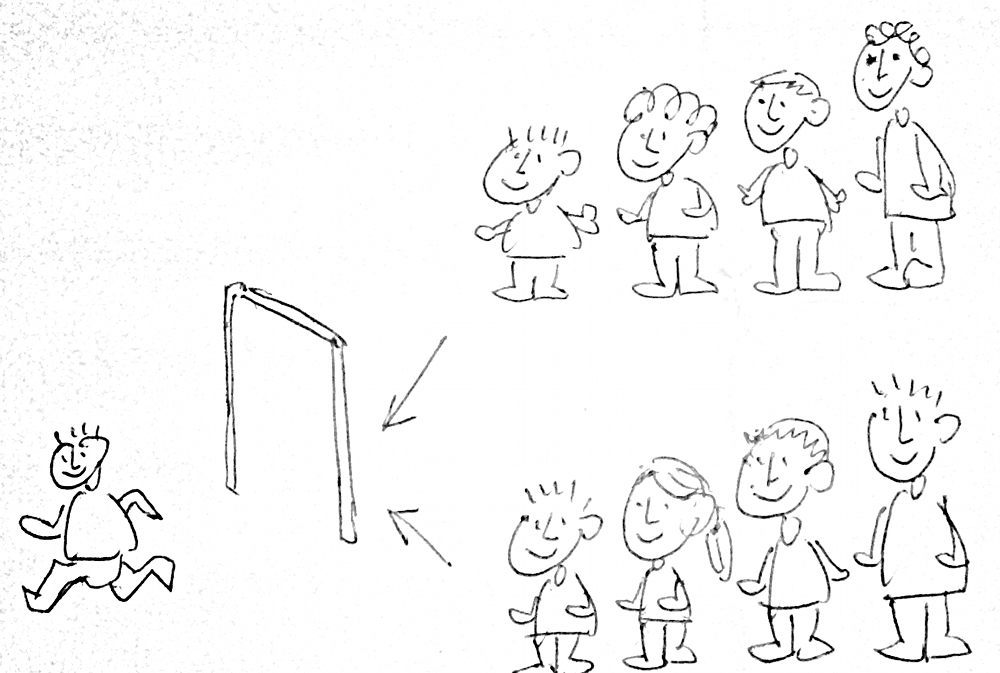
\includegraphics[scale=0.3]{img/merge.eps}
 \caption{Two lines of kids pass a door.}
 \label{fig:merge}
\end{figure}

Now let's ask the kids to pass a door one by one, every time there can be at least one kid
pass the door. The kids must pass this door in the order of their height. The one can't
pass the door before all the kids who are shorter than him/her.

Since the two lines of kids have already been `sorted', the solution is to ask the first
two kids, one from each line, compare their height, and let the shorter kid pass the door;
Then they repeat this step until one line is empty, after that, all the rest kids can
pass the door one by one. 

This idea can be formalized in the following equation.

\be
merge(A, B) = \left \{
  \begin{array}
  {r@{\quad:\quad}l}
  A & B = \Phi \\
  B & A = \Phi \\
  \{a_1\} \cup merge(A', B) & a_1 \leq b_1 \\
  \{b_1\} \cup merge(A, B') & otherwise
  \end{array}
\right. 
\ee

Where $a_1$ and $b_1$ are the first elements in list $A$ and $B$; $A'$ and $B'$ are the
rest elements except for the first ones respectively. The first two cases are trivial
edge cases. That merge one sorted list with an empty list results the same sorted list;
Otherwise, if both lists are non-empty, we take the first elements from the two lists,
compare them, and use the minimum as the first one of the result, then recursevely
merge the rest.

With $merge$ defined, the basic version of merge sort can be implemented like the following
Haskell example code.

\lstset{language=Haskell}
\begin{lstlisting}
msort [] = []
msort [x] = [x]
msort xs = merge (msort as) (msort bs) where
  (as, bs) = splitAt (length xs `div` 2) xs

merge xs [] = xs
merge [] ys = ys
merge (x:xs) (y:ys) | x <= y = x : merge xs (y:ys)
                    | x >  y = y : merge (x:xs) ys
\end{lstlisting}

Note that, the implemenation differs from the algorithm definition that it treats the singleton
list as trivial edge case.

Merge sort can also be realized impreatively. The basic version can be developed as the below algorithm.

\begin{algorithmic}
\Procedure{Sort}{$A$}
  \If{$|A| > 1$}
    \State $m \gets \lfloor \frac{|A|}{2} \rfloor$
    \State $X \gets$ \Call{Copy-Array}{$A[1...m]$}
    \State $Y \gets$ \Call{Copy-Array}{$A[m+1...|A|]$}
    \State \Call{Sort}{$X$}
    \State \Call{Sort}{$Y$}
    \State \Call{Merge}{$A, X, Y$}
  \EndIf
\EndProcedure
\end{algorithmic}

When the array to be sorted contains at least two elements, the non-trivial sorting process starts.
It first copy the first half to a new create array $A$, and the second half to a second new array $B$.
Recursively sort them by using merge sort algorithm; and finally merge the sorted result back to $A$.

This version uses the same amount of extra spaces of $A$. This is because the \textproc{Merge} algorithm
isn't in-place at the moment. We'll introduce the imperative in-place merge sort in later section.

The merge process almost does the samething as the functional definition. There is a verbose version
and a simplified version by using sentinel.

The verbose merge algorithm continous check the element from the two input arrays, pick the smaller one
and put it back to the result array $A$, it then advances along the arrays respectively until either
one input array is exhausted. After that, the algorithm append the rest of the elements in the other
input array to $A$.

\begin{algorithmic}
\Procedure{Merge}{$A, X, Y$}
  \State $i \gets 1, j\gets 1, k\gets 1$
  \State $m \gets |X|, n \gets |Y|$
  \While{$i \leq m \land j \leq n$}
    \If{$X[i] < Y[j]$}
      \State $A[k] \gets X[i]$
      \State $i \gets i + 1$
    \Else
      \State $A[k] \gets Y[j]$
      \State $j \gets j + 1$
    \EndIf
    \State $k \gets k + 1$
  \EndWhile
  \While{$i \leq m$}
    \State $A[k] \gets X[i]$
    \State $k \gets k + 1$
    \State $i \gets i + 1$
  \EndWhile
  \While{$j \leq n$}
    \State $A[k] \gets Y[j]$
    \State $k \gets k + 1$
    \State $j \gets j + 1$
  \EndWhile
\EndProcedure
\end{algorithmic}

Altough this algorithm is a bit verbose, it can be short in some programming environment with enough tools
to manipulate array. The following Python program is an example.

\lstset{language=Python}
\begin{lstlisting}
def msort(xs):
    n = len(xs)
    if n > 1:
        ys = [x for x in xs[:n/2]]
        zs = [x for x in xs[n/2:]]
        ys = msort(ys)
        zs = msort(zs)
        xs = merge(xs, ys, zs)
    return xs

def merge(xs, ys, zs):
    i = 0
    while ys != [] and zs != []:
        xs[i] = ys.pop(0) if ys[0] < zs[0] else zs.pop(0)
        i = i + 1
    xs[i:] = ys if ys !=[] else zs
    return xs
\end{lstlisting}

\subsubsection{Performance}
Before dive into the improvement of this basic version, let's analyze the performance of merge sort.
The algorithm contains two steps, divide step, and merge step. In divide step, the sequence to be 
sorted is always divided into two sub sequences with the same length. If we draw a similar partition tree
as what we did for quick sort, it can be found this tree is a perfect balanced binary tree as shown in
figure \ref{fig:qsort-best}. Thus the height of this tree is $O(\lg N)$. It means the recursion depth
of merge sort is bound to $O(\lg N)$. Merge happens in every level. It's intuitive to analyze the
merge algorithm, that it compare elements from two input sequences in pairs, after one sequence is fully examined
the rest one is copied one by one to the result, thus it's a linear algorithm proportion to the length of 
the sequence. Based on this facts, denote $T(N)$ is the time for sort the sequence with length $N$,
we can write the recursive time cost as below.

\be
\renewcommand*{\arraystretch}{2}
\begin{array}{rl}
T(N) & = \displaystyle T(\frac{N}{2}) + T(\frac{N}{2}) + c N \\
     & = \displaystyle 2 T(\frac{N}{2}) + c N
\end{array}
\ee

It states that the cost consists of three parts: merge sort the first half takes $T(\frac{N}{2})$, 
merge sort the second half takes also $T(\frac{N}{2})$, merge the two results takes $c N$, where $c$
is some constant. Solve this equation gives the result as $O(N \lg N)$.

Note that, this performance doesn't vary in all cases, as merge sort alwasy uniformed divids the input.

Another significant performance indicator is space occupation. However, it varies a lot in different
merge sort implementation. The detail space bounds analysis will be explained in every detailed variants
later.

For the basic imperative merge sort, observe that it demands same amount of spaces as the input array
in every recursion, copies the original elements to them for recusive sort, and these spaces can
be released after this level of recusrion. So the peak space requirement happens when the recursion
enters to the deepest level, which is $O(N \lg N)$.

The functional merge sort consume much less than this amount, because the underlying data structure
of the sequence is linked-list. Thus it needn't extra spaces for merge\footnote{The complex effects
casued by lazy evaluation is ignored here, please refer to \cite{algo-fp} for detail}. 
The only spaces requirement is for book-keeping the stack for recursive calls. This can be
seen in the later explaination of even-odd split algorithm.

\subsubsection{Minor improvement}

We'll next improve the basic merge sort bit by bit for both the functional and imperative realizations.
The first observation is that the imperative merge algorithm is a bit verbose. \cite{CLRS} presents
an elegant simplification by using positive $\infty$ as the sentinel. That we append $\infty$ as
the last element in both ordered arrays for merging\footnote{For sorting in monotonic non-increasing order,
$-\infty$ can be used instead}. Thus we needn't test which array is not exhausted, and append it 
to the end of the result.

TODO: illustrate this idea by figures

\begin{algorithmic}
\Procedure{Merge}{$A, X, Y$}
  \State \Call{Append}{$X, \infty$}
  \State \Call{Append}{$Y, \infty$}
  \State $i \gets 1, j\gets 1$
  \For{$k \gets$ from 1 to $|A|$}
    \If{$X[i] < Y[j]$}
      \State $A[k] \gets X[i]$
      \State $i \gets i + 1$
    \Else
      \State $A[k] \gets Y[j]$
      \State $j \gets j + 1$
    \EndIf
  \EndFor
\EndProcedure  
\end{algorithmic}

The following ANSI C program illustrated this idea. It embeds the merge inside. \verb|INF| is defined
as a big constant number with the same type of \verb|Key|. Where the type can either defined elsewhere
or we can abstract the type information by passing the comparator as parameter. We skip these
implementation and language details here.

\lstset{language=C}
\begin{lstlisting}
void msort(Key* xs, int l, int u) {
    int i, j, m;
    Key *as, *bs;
    if (u - l > 1) {
        m = l + (u - l) / 2;  /* avoid int overflow */
        msort(xs, l, m);
        msort(xs, m, u);
        as = (Key*) malloc(sizeof(Key) * (m - l + 1));
        bs = (Key*) malloc(sizeof(Key) * (u - m + 1));
        memcpy((void*)as, (void*)(xs + l), sizeof(Key) * (m - l));
        memcpy((void*)bs, (void*)(xs + m), sizeof(Key) * (u - m));
        as[m - l] = bs[u - m] = INF;
        for (i = j = 0; l < u; ++l)
            xs[l] = as[i] < bs[j] ? as[i++] : bs[j++];
        free(as);
        free(bs);
    }
}
\end{lstlisting}

Running this program takes much more time than the quick sort. Besides the major reason we'll explain later,
one problem is that this version frequently allocates and releases extra memories for merging. While memory
allocation is one of the well known bottle-neck in real world as mentioned by Bentley in \cite{pearls}.
One solution to address this issue is to allocate another array with the same size to the original one
as working area. The recursive sort for the first and second halves needn't allocate any more
extra spaces, but using the working area when merging. Finally, the algorithm copies
the merged result back.

This idea can be expressed as the following modified algorithm.

\begin{algorithmic}
\Procedure{Sort}{A}
  \State $B \gets $ \Call{Create-Array}{$|A|$}
  \State \Call{Sort'}{$A, B, 1, |A|$}
\EndProcedure
\Statex
\Procedure{Sort'}{$A, B, l, u$}
  \If{$u - l > 0$}
    \State $m \gets \lfloor \frac{l + u}{2} \rfloor$
    \State \Call{Sort'}{$A, B, l, m$}
    \State \Call{Sort'}{$A, B, m + 1, u$}
    \State \Call{Merge'}{$A, B, l, m, u$}
  \EndIf
\EndProcedure
\end{algorithmic}

This algorithm duplicates another array, and pass it along with the original array to be sorted
to \textproc{Sort'} algorithm. In real implementation, this working area should be released
either manually, or by some automatic tool such as GC (Gabbage collection).
The modified algorithm \textproc{Merge'} also accepts a working area as parameter.

\begin{algorithmic}
\Procedure{Merge'}{$A, B, l, m, u$}
  \State $i \gets l, j \gets m + 1, k \gets l$
  \While{$i \leq m \land j \leq u$}
    \If{$A[i] < A[j]$}
      \State $B[k] \gets A[i]$
      \State $i \gets i + 1$
    \Else
      \State $B[k] \gets A[j]$
      \State $j \gets j + 1$
    \EndIf
    \State $k \gets k + 1$
  \EndWhile
  \While{$i \leq m$}
    \State $B[k] \gets A[i]$
    \State $k \gets k + 1$
    \State $i \gets i + 1$
  \EndWhile
  \While{$j \leq u$}
    \State $B[k] \gets A[j]$
    \State $k \gets k + 1$
    \State $j \gets j + 1$
  \EndWhile
  \For{$i \gets$ from $l$ to $u$} \Comment{Copy back}
    \State $A[i] \gets B[i]$
  \EndFor
\EndProcedure
\end{algorithmic}

By using this minor improvement, the space requirement reduced to $O(N)$ from $O(N \lg N)$.
The following ANSI C program implements this minor improvement. For illustration purpose,
we manually copy the merged result back to the original array in a loop. This can also
be realized by using standard library provided tool, such as \verb|memcpy|.

\lstset{language=C}
\begin{lstlisting}
void merge(Key* xs, Key* ys, int l, int m, int u) {
    int i, j, k;
    i = k = l; j = m;
    while (i < m && j < u)
        ys[k++] = xs[i] < xs[j] ? xs[i++] : xs[j++];
    while (i < m)
        ys[k++] = xs[i++];
    while (j < u)
        ys[k++] = xs[j++];
    for(; l < u; ++l)
        xs[l] = ys[l];
}

void msort(Key* xs, Key* ys, int l, int u) {
    int m;
    if (u - l > 1) {
        m = l + (u - l) / 2;
        msort(xs, ys, l, m);
        msort(xs, ys, m, u);
        merge(xs, ys, l, m, u);
    }
}

void sort(Key* xs, int l, int u) {
    Key* ys = (Key*) malloc(sizeof(Key) * (u - l));
    kmsort(xs, ys, l, u);
    free(ys);
}
\end{lstlisting}

This new version runs faster than the previous one. In my test machine, it speeds up about 20\% to 25\% when sorting
100,000 randomly generated numbers.

The basic functional merge sort can also be fine tuned. Observe that, it splits the list at the middle point. However,
as the underlying data structure to represent list is singly linked-list, random access at a given position is
a linear operation (refer to appendix for detail). Alternatively, one can split the list in an even-odd manner.
That all the elements in even position are collected in one sub list, while all the odd elements are collected
in another. As for any lists, there are either same amount of elements in even and odd positions, or they
differ by one. So this divide strategy always leads to well spliting, thus the performance can be ensured
to be $O(N \lg N)$ in all cases.

The even-odd spliting algorithm can be defined as below.

\be
split(L) = \left \{
  \begin{array}
  {r@{\quad:\quad}l}
  (\Phi, \Phi) & L = \Phi \\
  (\{ l_1 \}, \Phi) & |L| = 1 \\
  (\{ l_1 \} \cup A, \{ l_2 \} \cup B) & otherwise, (A, B) = split(L'')
  \end{array}
\right.
\ee

When the list is empty, the split result are two empty lists; If there is only one element in the list, we put this
singleton element, which is at position 1, to the odd sub list, the even sub list is empty; Otherwise, it means
there are at least two elements in the list, We pick the first one to the odd sub list, the second one to the
even sub list, and recursively split the rest elements.

All the other functions are kept same, the modified Haskell program is given as the following.

\lstset{language=Haskell}
\begin{lstlisting}
split [] = ([], [])
split [x] = ([x], [])
split (x:y:xs) = (x:xs', y:ys') where (xs', ys') = split xs
\end{lstlisting}

TODO: provied a imperative singly linked-list ver.

\section{In-place merge sort}
One drawback for the imperative merge sort is that it requires extra spaces for merging, the basic version without
any optimization needs $O(N \lg N)$ in peak time, and the one by allocating a working area needs $O(N)$.

It's nature for people to seek the in-place version merge sort, which can reuse the original array without allocating
any extra spaces. In this section, we'll introduce some solutions to realize imperative in-place merge sort.

\subsection{Naive in-place merge}
The first idea is straightforward. As illustrated in figure \ref{fig:merge-in-place-naive}, sub list $A$, and $B$
are sorted, when performs in-place merge, the variant ensures that all elements before $i$ are merged, so that
they are in non-decreasing order; every time we compare the $i$-th and the $j$-th elements. If the $i$-th is less
than the $j$-th, the marker $i$ just advances one step to the next. This is the easy case. Otherwise, it
means that the $j$-th element is the next merge result, which should be put in front of the $i$-th. In order
to achieve this, all elements between $i$ and $j$, including the $i$-th should be shift to the end by one cell.
We repeat this process till all the elements in $A$ and $B$ are put to the correct positions.

\begin{figure}[htbp]
 \centering
 \includegraphics[scale=0.8]{img/merge-in-place-naive.ps}
 \caption{Naive in-place merge}
 \label{fig:merge-in-place-naive}
\end{figure}

\begin{algorithmic}
\Procedure{Merge}{$A, l, m, u$}
  \While{$l \leq m \land m \leq u$}
    \If{$A[l] < A[m]$}
      \State $l \gets l + 1$
    \Else
      \State $x \gets A[m]$
      \For{$i \gets m $ down-to $l+1$} \Comment{Shift}
        \State $A[i] \gets A[i-1]$
      \EndFor
      \State $A[l] \gets x$
    \EndIf
  \EndWhile
\EndProcedure
\end{algorithmic}

However, this naive solution downgrades merge sort overall performance to quadratic $O(N^2)$! This is because
that array shifting is a linear operation, which is proportion to the length of elements in 
the first sorted sub array which haven't been compared so far. 

The following ANSI C program based on this algorithm runs very slow, that it takes about 12 times slow than
the previous version when sorting 10,000 random numbers.

\lstset{language=C}
\begin{lstlisting}
void naive_merge(Key* xs, int l, int m, int u) {
    int i; Key y;
    for(; l < m && m < u; ++l)
        if (!(xs[l] < xs[m])) {
            y = xs[m++];
            for (i = m - 1; i > l; --i) /* shift */
                xs[i] = xs[i-1];
            xs[l] = y;
        }
}

void msort3(Key* xs, int l, int u) {
    int m;
    if (u - l > 1) {
        m = l + (u - l) / 2;
        msort3(xs, l, m);
        msort3(xs, m, u);
        naive_merge(xs, l, m, u);
    }
}  
\end{lstlisting}

\subsection{in-place working area}

In order to implement the in-place merge sort in $O(N \lg N)$ time, when sorting a sub array, the rest part of 
the array must be reused as working area for merging. As the elements stored in the working area, will be sorted
later, they can't be overwritten. We can modify the previous algorithm, which douplicate an extra spaces for merging
a bit to achieve this. The idea is that, every time when we compare the first elements in the two sorted sub
array, if we want to put the less element to the target position in the working area, we in-turn exchange what
sored in the working area with this element. Thus after merging the two sub arrays store what the working area
previously contains. This idea can be illustrated in figure \ref{fig:merge_workarea}.

\begin{figure}[htbp]
 \centering
 \includegraphics[scale=0.8]{img/merge-workarea.ps}
 \caption{Merge without overwritting work area.}
 \label{fig:merge-workarea}
\end{figure}

In our algorithm, both the two sorted sub array, and the working area for merging are all part of the 
origianl array to be sorted. we need pass the following arguments when merging: the start points and end
points of the sorted sub arrays, which can be represented as ranges; and the start point of the working
area. The following algorithm description for example, use $[a, b)$ to indicate the range include $a$, 
exclude $b$. It merges sorted range $[i, m)$ and range $[j, n)$ to work area starts from $k$.

\begin{algorithmic}
\Procedure{Merge}{$A, [i, m), [j, n), k$}
  \While{$i < m \land j < n$}
    \If{$A[i] < A[j]$}
      \State \textproc{Exchange} $A[k] \leftrightarrow A[i]$
      \State $i \gets i + 1$
    \Else
      \State \textproc{Exchange} $A[k] \leftrightarrow A[j]$
      \State $j \gets j + 1$
    \EndIf
    \State $k \gets k + 1$
  \EndWhile
  \While{$i < m$}
    \State \textproc{Exchange} $A[k] \leftrightarrow A[i]$
    \State $i \gets i + 1$
    \State $k \gets k + 1$
  \EndWhile
  \While{$j < m$}
    \State \textproc{Exchange} $A[k] \leftrightarrow A[j]$
    \State $j \gets j + 1$
    \State $k \gets k + 1$
  \EndWhile
\EndProcedure
\end{algorithmic}

Note that, the following two constraints must be satisfied when merging:

\begin{enumerate}
\item The work area should be within the bound of the array. In other words, it should be big 
enough to hold elements exchanged in without causing any out-of-bound error;
\item The work area can be overlapped with either of the two sorted arrays, however, it should
be ensured that there are not any unmerged elements being overwritten;
\end{enumerate}

This algorithm can be implemented in ANSI C as the following example.

\lstset{language=C}
\begin{lstlisting}
void wmerge(Key* xs, int i, int m, int j, int n, int w) {
    while (i < m && j < n)
        swap(xs, w++, xs[i] < xs[j] ? i++ : j++);
    while (i < m)
        swap(xs, w++, i++);
    while (j < n)
        swap(xs, w++, j++);
}  
\end{lstlisting}

With this merging algorithm defined, it's easy to imagine a solution, which can sort
half of the array; The next question is, how to deal with the rest of the unsort part
stored in work area as shown in figure \ref{fig:merge-in-place-start}?

\begin{figure}[htbp]
 \centering
 \includegraphics[scale=0.8]{img/merge-in-place-start.ps}
 \caption{Half of the array is soreted.}
 \label{fig:merge-in-place-start}
\end{figure}

One intuitive idea is to recursive sort another half of the working area, thus there are
only $\frac{1}{4}$ elements haven't been sorted yet. Which is shown in figure \ref{fig:merge-in-place-quater}.
The key point at this stage is that we must merge the sorted $\frac{1}{4}$ elements $B$
with the sorted $\frac{1}{2}$ elements $A$ sooner or later.

\begin{figure}[htbp]
 \centering
 \includegraphics[scale=0.8]{img/merge-in-place-quater.ps}
 \caption{$A$ and $B$ must be merged at sometime.}
 \label{fig:merge-in-place-quater}
\end{figure}

Is the working area left, which only holds $\frac{1}{4}$ elements, big enough to merge
$A$ and $B$? Unfortunately, it isn't in the setting shown in figure \ref{fig:merge-in-place-quater}.

However, the second constraint mentioned before gives us a hint, that we can exploit
it by arranging the working area to overlap with either sub array if we can ensure the
merging sequence that the unmerged elements won't be overwritten.

Actually, instead of sorting the second half of the working area, we can sort the first
half, and put the working area between the two sorted arrays as shown in figure \ref{fig:merge-in-place-setup} (a).
This setup effects arrange the work area overlap with the sub array $A$. This idea
is proposed in \cite{msort-in-place}.

\begin{figure}[htbp]
 \centering
 \subfloat[]{\includegraphics[scale=0.8]{img/merge-in-place-setup.ps}} \\
 \subfloat[]{\includegraphics[scale=0.8]{img/merge-in-place-merged-quater.ps}}
 \caption{Merge $A$ and $B$ with a work area.}
 \label{fig:merge-in-place-setup}
\end{figure}

Let's consider two extreme cases:

\begin{enumerate}
\item All the elements in $B$ are less than any elements in $A$. In this case, the merge algorithm
finally moves the whole contents of $B$ to the working area; the cells of $B$ holds what previously
stored in the workarea; As the size of area is as same as $B$, it's OK for exchange their contents;
\item All the elements in $A$ are less than any elements in $B$. In this case, the merge algorithm
continously exchanges elements between $A$ and the workarea. After all the previous $\frac{1}{4}$ 
cells in the work area are filled with elements from $A$, the algorithm starts to overwrite the
first half of $A$, fortunately, the contents being overwritten are not those unmerged elements.
The work area is in effect advances towards the end of the array, and finally moves to the right
side; From this time point, the merge algorithm start exchange contents in $B$ with the work area.
The result is that the work area moves to the right most side which is shown in figure \ref{fig:merge-in-place-setup} (b).
\end{enumerate}

We can repeat this step, that always sort the second half of the unsorted part, and exchange
the sorted sub array to the first half as working area. Thus we keep reducing the working area 
from $\frac{1}{2}$ of the array, $\frac{1}{4}$
of the array, $\frac{1}{8}$ of the array, ... The scale of the merge problem keeps reducing.
When there is only one element left in the working area, we needn't sort it any more since
the singleton array is sorted by nature. Merge a singleton array to the other is equivellent
to insert the element. In practice, the algorithm can finalize the last few 
elements by switching to insertion sort.

The who algorithm can be described as the following.

\begin{algorithmic}
\Procedure{Sort}{$A, l, u$}
  \If{$u - l > 0$}
    \State $m \gets \lfloor \frac{l + u}{2} \rfloor$
    \State $w \gets l + u - m$
    \State \Call{Sort'}{$A, l, m, w$} \Comment{The second half contains sorted elements}
    \While{$w - l > 1$}
      \State $u' \gets w$
      \State $w \gets \lceil \frac{l + u'}{2} \rceil$ \Comment{Ensure the working area is big enough}
      \State \Call{Sort'}{$A, w, u', l$} \Comment{The first half holds the sorted elements}
      \State \Call{Merge}{$A, [l, l + u' - w], [u', u], w$}
    \EndWhile
    \For{$i \gets w$ down-to $l$} \Comment{Switch to insertion sort}
      \State $j \gets i$
      \While{$j \leq u \land A[j] < A[j-1]$}
        \State \textproc{Exchange} $A[j] \leftrightarrow A[j-1]$
        \State $j \gets j + 1$
      \EndWhile
    \EndFor
  \EndIf
\EndProcedure
\end{algorithmic}

Note that in order to satisfy the first constrait, we must ensure the working area is big enough to hold
all exhanged in elements, that's way we round it by ceiling when sort the second half of the working area.
Note that we actually pass the ranges including the end points to the algorithm \textproc{Merge}.

Next, we develope a \text{Sort'} algorithm, which mutually recursive call \text{Sort} and exhange the result
to the working area.

\begin{algorithmic}
\Procedure{Sort'}{$A, l, u, w$}
  \If{$u - l > 0$}
    \State $m \gets \lfloor \frac{l + u}{2} \rfloor$
    \State \Call{Sort}{$A, l, m$}
    \State \Call{Sort}{$A, m+1, u$}
    \State \Call{Merge}{$A, [l, m], [m+1, u], w$}
  \Else \Comment{Exhange all elements to the work area}
    \While{$l \leq u$}
      \State \textproc{Exchange} $A[l] \leftrightarrow A[w]$
      \State $l \gets l + 1$
      \State $w \gets w + 1$
    \EndWhile
  \EndIf
\EndProcedure
\end{algorithmic}

Different from the naive in-place sort, this algorithm doesn't shift the array during merging. The main
algorithm reduces the unsort part in sequence of $N/2, N/4, N/8, ...$, it takes $O(\lg N)$ steps to complete
sorting. In every step, It recurisve sort half of the rest elements, and perform linear time merging.

Denote the time cost of sorting $N$ elements as $T(N)$, we have the following equation.

\be
T(N) = T(\frac{N}{2}) + c \frac{N}{2} + T(\frac{N}{4}) + c \frac{3N}{4} + T(\frac{N}{8}) + c \frac{7N}{8} + ...
\ee

Solving this equation by using telescope method, get the result $O(N \lg N)$. The detailed process is
left as exercise to the reader.

The following ANSI C code complete the implementation by using the example \verb|wmerge| program given 
above.

\lstset{language=C}
\begin{lstlisting}
void imsort(Key* xs, int l, int u);

void wsort(Key* xs, int l, int u, int w) {
    int m;
    if (u - l > 1) {
        m = l + (u - l) / 2;
        imsort(xs, l, m);
        imsort(xs, m, u);
        wmerge(xs, l, m, m, u, w);
    }
    else
        while (l < u)
            swap(xs, l++, w++);
}

void imsort(Key* xs, int l, int u) {
    int m, n, w;
    if (u - l > 1) {
        m = l + (u - l) / 2;
        w = l + u - m;
        wsort(xs, l, m, w); /* the last half contains sorted elements */
        while (w - l > 2) {
            n = w;
            w = l + (n - l + 1) / 2; /* ceiling */
            wsort(xs, w, n, l);  /* the first half contains sorted elements */
            wmerge(xs, l, l + n - w, n, u, w);
        }
        for (n = w; n > l; --n) /*switch to insertion sort*/
            for (m = n; m < u && xs[m] < xs[m-1]; ++m)
                swap(xs, m, m - 1);
    }
}
\end{lstlisting}

However, this program doesn't run faster than version we developed in previous section, which double
the array in advance as working area. In my machine, it is about 60\% slower when sorting 100,000 random 
numbers due to many swap operations.

\subsection{In-place merge sort V.S. linked-list merge sort}

The in-place merge sort is still a live area for research. In order to save the extra spaces for merging,
some overhead has be introduced, which increase the complecxity of the merge sort algorithm. However, if
the underlying data structure isn't array, but linked list, merge can be achieved without any extra spaces
as shown in the even-odd functional merge sort algorithm presented in previous section.

In order to make it clearer, we can develop a purely imperative linked-list merge sort solution.
The linked-list can be defined as a record type as shown in appendix A like below.

\lstset{language=C}
\begin{lstlisting}
struct Node {
    Key key;
    struct Node* next;
};  
\end{lstlisting}

We can define an auxiliary function for node linking. Assume the list to be linked isn't empty, it
can be implemented as the following.

\lstset{language=C}
\begin{lstlisting}
struct Node* link(struct Node* xs, struct Node* ys) {
    xs->next = ys;
    return xs;
}  
\end{lstlisting}

One method to realize the imperative even-odd splitting, is to initialize two empty sub lists.
Then iterate the list to be splitted. Every time, we link the current node in front of the
first sub list, then exchange the two sub lists. So that, the second sub list will be linked
at the next time iteration. This idea can be illustrated as below.

\begin{algorithmic}
\Function{Split}{$L$}
  \State $(A, B) \gets (\Phi, \Phi)$
  \While{$L \neq \Phi$}
    \State $p \gets L$
    \State $L \gets $ \Call{Next}{$L$}
    \State $A \gets $ \Call{Link}{$p, A$}
    \State \textproc{Exchange} $A \leftrightarrow B$
  \EndWhile
  \State \Return $(A, B)$
\EndFunction
\end{algorithmic}

The following example ANSI C program implements this splitting algorithm embedded.

\lstset{language=C}
\begin{lstlisting}
struct Node* msort(struct Node* xs) {
    struct Node *p, *as, *bs;
    if (!xs || !xs->next) return xs;

    as = bs = NULL;
    while(xs) {
        p = xs;
        xs = xs->next;
        as = link(p, as);
        swap(as, bs);
    }
    as = msort(as);
    bs = msort(bs);
    return merge(as, bs);
}  
\end{lstlisting}

The only thing left is to develop the imperative merging algorithm for linked-list. The idea
is quite similar to the array merging version. As long as neither of the sub lists is exhausted,
we pick the less one, and append it to the result list. After that, it just need link the
non-empty one to the tail the result, but not a looping for copying. It's need some carefulness
to initiaize the result list, as its head node is the less one among the two sub lists.
One simple method is to use a dummy sentinel head, and drop it before returning. This implementation
detail can be given as the following.

\lstset{language=C}
\begin{lstlisting}
struct Node* merge(struct Node* as, struct Node* bs) {
    struct Node s, *p;
    p = &s;
    while (as && bs) {
        if (as->key < bs->key) {
            link(p, as);
            as = as->next;
        }
        else {
            link(p, bs);
            bs = bs->next;
        }
        p = p->next;
    }
    if (as)
        link(p, as);
    if (bs)
        link(p, bs);
    return s.next;
}  
\end{lstlisting}

\begin{Exercise}
\begin{itemize}
\item Proof the performance of in-place merge sort is bound to $O(N \lg N)$.
\end{itemize}
\end{Exercise}

\section{Nature merge sort}
Knuth gives another way to interpret the idea of divide and conquer merge sort by using the example
of burning a candle in both ends \cite{TAOCP}. This leads to the nature merge sort algorithm.

that we can double the size of the array to be sorted.
The first half of this new array contains elements we are sorting, the second half is used as
working area for merging. When we enter the next recursion, we switch to use the second half
for sorting, and use the first half as working area; Such switching happends repeatedly in
recursive calls. Finally, we copied all elements from the second half as the result.

TODO: illustrate this idea by using figure.

\section{Bottom-up merge sort}

\section{Short summary} 
From easy/hard partition, easy/hard merge point of view

TODO:

\begin{thebibliography}{99}

\bibitem{TAOCP}
Donald E. Knuth. ``The Art of Computer Programming, Volume 3: Sorting and Searching (2nd Edition)''. Addison-Wesley Professional; 2 edition (May 4, 1998) ISBN-10: 0201896850 ISBN-13: 978-0201896855

\bibitem{CLRS}
Thomas H. Cormen, Charles E. Leiserson, Ronald L. Rivest and Clifford Stein. 
``Introduction to Algorithms, Second Edition''. ISBN:0262032937. The MIT Press. 2001

\bibitem{qsort-impl}
Robert Sedgewick. ``Implementing quick sort programs''. Communication of ACM. Volume 21, Number 10. 1978. pp.847 - 857.

\bibitem{pearls}
Jon Bentley. ``Programming pearls, Second Edtion''. Addison-Wesley Professional; 1999. ISBN-13: 978-0201657883

\bibitem{3-way-part}
Jon Bentley, Douglas McIlroy. ``Engineering a sort function''. Software Practice and experience VOL. 23(11), 1249-1265 1993.

\bibitem{opt-qs}
Robert Sedgewick, Jon Bentley. ``Quicksort is optimal''. http://www.cs.princeton.edu/~rs/talks/QuicksortIsOptimal.pdf

\bibitem{fp-pearls}
Richard Bird. ``Pearls of functional algorithm design''. Cambridge University Press. 2010. ISBN, 1139490605, 9781139490603

\bibitem{algo-fp}
Fethi Rabhi, Guy Lapalme. ``Algorithms: a functional programming approach''. Second edition. Addison-Wesley, 1999. ISBN: 0201-59604-0

\bibitem{slpj}
Simon Peyton Jones. ``The Impelementation of functional programming languages''. Prentice-Hall International, 1987. ISBN: 0-13-453333-X

\bibitem{msort-in-place}
Jyrki Katajainen, Tomi Pasanen, Jukka Teuhola. ``Practical in-place mergesort''. Nordic Journal of Computing, 1996.

\bibitem{wiki-qs}
Wikipedia. ``Quicksort''. http://en.wikipedia.org/wiki/Quicksort

\bibitem{wiki-sweak-order}
Wikipedia. ``Strict weak order''. http://en.wikipedia.org/wiki/Strict\_weak\_order

\bibitem{wiki-total-order}
Wikipedia. ``Total order''. http://en.wokipedia.org/wiki/Total\_order

\bibitem{wiki-harmonic}
Wikipedia. ``Harmonic series (mathematics)''. http://en.wikipedia.org/wiki/Harmonic\_series\_(mathematics)

\end{thebibliography}

\ifx\wholebook\relax\else
\end{document}
\fi
